% Options for packages loaded elsewhere
\PassOptionsToPackage{unicode}{hyperref}
\PassOptionsToPackage{hyphens}{url}
%
\documentclass[
  ignorenonframetext,
]{beamer}
\usepackage{pgfpages}
\setbeamertemplate{caption}[numbered]
\setbeamertemplate{caption label separator}{: }
\setbeamercolor{caption name}{fg=normal text.fg}
\beamertemplatenavigationsymbolsempty
% Prevent slide breaks in the middle of a paragraph
\widowpenalties 1 10000
\raggedbottom
\setbeamertemplate{part page}{
  \centering
  \begin{beamercolorbox}[sep=16pt,center]{part title}
    \usebeamerfont{part title}\insertpart\par
  \end{beamercolorbox}
}
\setbeamertemplate{section page}{
  \centering
  \begin{beamercolorbox}[sep=12pt,center]{part title}
    \usebeamerfont{section title}\insertsection\par
  \end{beamercolorbox}
}
\setbeamertemplate{subsection page}{
  \centering
  \begin{beamercolorbox}[sep=8pt,center]{part title}
    \usebeamerfont{subsection title}\insertsubsection\par
  \end{beamercolorbox}
}
\AtBeginPart{
  \frame{\partpage}
}
\AtBeginSection{
  \ifbibliography
  \else
    \frame{\sectionpage}
  \fi
}
\AtBeginSubsection{
  \frame{\subsectionpage}
}
\usepackage{amsmath,amssymb}
\usepackage{lmodern}
\usepackage{iftex}
\ifPDFTeX
  \usepackage[T1]{fontenc}
  \usepackage[utf8]{inputenc}
  \usepackage{textcomp} % provide euro and other symbols
\else % if luatex or xetex
  \usepackage{unicode-math}
  \defaultfontfeatures{Scale=MatchLowercase}
  \defaultfontfeatures[\rmfamily]{Ligatures=TeX,Scale=1}
\fi
% Use upquote if available, for straight quotes in verbatim environments
\IfFileExists{upquote.sty}{\usepackage{upquote}}{}
\IfFileExists{microtype.sty}{% use microtype if available
  \usepackage[]{microtype}
  \UseMicrotypeSet[protrusion]{basicmath} % disable protrusion for tt fonts
}{}
\makeatletter
\@ifundefined{KOMAClassName}{% if non-KOMA class
  \IfFileExists{parskip.sty}{%
    \usepackage{parskip}
  }{% else
    \setlength{\parindent}{0pt}
    \setlength{\parskip}{6pt plus 2pt minus 1pt}}
}{% if KOMA class
  \KOMAoptions{parskip=half}}
\makeatother
\usepackage{xcolor}
\newif\ifbibliography
\usepackage{color}
\usepackage{fancyvrb}
\newcommand{\VerbBar}{|}
\newcommand{\VERB}{\Verb[commandchars=\\\{\}]}
\DefineVerbatimEnvironment{Highlighting}{Verbatim}{commandchars=\\\{\}}
% Add ',fontsize=\small' for more characters per line
\usepackage{framed}
\definecolor{shadecolor}{RGB}{248,248,248}
\newenvironment{Shaded}{\begin{snugshade}}{\end{snugshade}}
\newcommand{\AlertTok}[1]{\textcolor[rgb]{0.94,0.16,0.16}{#1}}
\newcommand{\AnnotationTok}[1]{\textcolor[rgb]{0.56,0.35,0.01}{\textbf{\textit{#1}}}}
\newcommand{\AttributeTok}[1]{\textcolor[rgb]{0.77,0.63,0.00}{#1}}
\newcommand{\BaseNTok}[1]{\textcolor[rgb]{0.00,0.00,0.81}{#1}}
\newcommand{\BuiltInTok}[1]{#1}
\newcommand{\CharTok}[1]{\textcolor[rgb]{0.31,0.60,0.02}{#1}}
\newcommand{\CommentTok}[1]{\textcolor[rgb]{0.56,0.35,0.01}{\textit{#1}}}
\newcommand{\CommentVarTok}[1]{\textcolor[rgb]{0.56,0.35,0.01}{\textbf{\textit{#1}}}}
\newcommand{\ConstantTok}[1]{\textcolor[rgb]{0.00,0.00,0.00}{#1}}
\newcommand{\ControlFlowTok}[1]{\textcolor[rgb]{0.13,0.29,0.53}{\textbf{#1}}}
\newcommand{\DataTypeTok}[1]{\textcolor[rgb]{0.13,0.29,0.53}{#1}}
\newcommand{\DecValTok}[1]{\textcolor[rgb]{0.00,0.00,0.81}{#1}}
\newcommand{\DocumentationTok}[1]{\textcolor[rgb]{0.56,0.35,0.01}{\textbf{\textit{#1}}}}
\newcommand{\ErrorTok}[1]{\textcolor[rgb]{0.64,0.00,0.00}{\textbf{#1}}}
\newcommand{\ExtensionTok}[1]{#1}
\newcommand{\FloatTok}[1]{\textcolor[rgb]{0.00,0.00,0.81}{#1}}
\newcommand{\FunctionTok}[1]{\textcolor[rgb]{0.00,0.00,0.00}{#1}}
\newcommand{\ImportTok}[1]{#1}
\newcommand{\InformationTok}[1]{\textcolor[rgb]{0.56,0.35,0.01}{\textbf{\textit{#1}}}}
\newcommand{\KeywordTok}[1]{\textcolor[rgb]{0.13,0.29,0.53}{\textbf{#1}}}
\newcommand{\NormalTok}[1]{#1}
\newcommand{\OperatorTok}[1]{\textcolor[rgb]{0.81,0.36,0.00}{\textbf{#1}}}
\newcommand{\OtherTok}[1]{\textcolor[rgb]{0.56,0.35,0.01}{#1}}
\newcommand{\PreprocessorTok}[1]{\textcolor[rgb]{0.56,0.35,0.01}{\textit{#1}}}
\newcommand{\RegionMarkerTok}[1]{#1}
\newcommand{\SpecialCharTok}[1]{\textcolor[rgb]{0.00,0.00,0.00}{#1}}
\newcommand{\SpecialStringTok}[1]{\textcolor[rgb]{0.31,0.60,0.02}{#1}}
\newcommand{\StringTok}[1]{\textcolor[rgb]{0.31,0.60,0.02}{#1}}
\newcommand{\VariableTok}[1]{\textcolor[rgb]{0.00,0.00,0.00}{#1}}
\newcommand{\VerbatimStringTok}[1]{\textcolor[rgb]{0.31,0.60,0.02}{#1}}
\newcommand{\WarningTok}[1]{\textcolor[rgb]{0.56,0.35,0.01}{\textbf{\textit{#1}}}}
\usepackage{graphicx}
\makeatletter
\def\maxwidth{\ifdim\Gin@nat@width>\linewidth\linewidth\else\Gin@nat@width\fi}
\def\maxheight{\ifdim\Gin@nat@height>\textheight\textheight\else\Gin@nat@height\fi}
\makeatother
% Scale images if necessary, so that they will not overflow the page
% margins by default, and it is still possible to overwrite the defaults
% using explicit options in \includegraphics[width, height, ...]{}
\setkeys{Gin}{width=\maxwidth,height=\maxheight,keepaspectratio}
% Set default figure placement to htbp
\makeatletter
\def\fps@figure{htbp}
\makeatother
\setlength{\emergencystretch}{3em} % prevent overfull lines
\providecommand{\tightlist}{%
  \setlength{\itemsep}{0pt}\setlength{\parskip}{0pt}}
\setcounter{secnumdepth}{-\maxdimen} % remove section numbering
\ifLuaTeX
  \usepackage{selnolig}  % disable illegal ligatures
\fi
\IfFileExists{bookmark.sty}{\usepackage{bookmark}}{\usepackage{hyperref}}
\IfFileExists{xurl.sty}{\usepackage{xurl}}{} % add URL line breaks if available
\urlstyle{same} % disable monospaced font for URLs
\hypersetup{
  pdftitle={ECON 1190: Applied Econometrics 2: Module 6: Regression Discontinuity},
  pdfauthor={Claire Duquennois},
  hidelinks,
  pdfcreator={LaTeX via pandoc}}

\title{ECON 1190: Applied Econometrics 2:\\
Module 6: Regression Discontinuity}
\author{Claire Duquennois}
\date{}

\begin{document}
\frame{\titlepage}

\begin{frame}{Regression discontinuity research designs}
\protect\hypertarget{regression-discontinuity-research-designs}{}
Introduced in other fields as far back as the 1960s.

Gain popularity in economics in the past 20 years or so as economists:

\begin{itemize}
\item
  increasingly focus on causal inference
\item
  large administrative datasets became more widely available
\end{itemize}

When correctly applied, RD designs are very transparent in how they
achieve causal identification which makes them very appealing.
\end{frame}

\begin{frame}{Regression discontinuity research designs}
\protect\hypertarget{regression-discontinuity-research-designs-1}{}
RD designs leverage the researchers knowledge of a rule or policy that
determines treatment.

Identification comes from how some rules are applied in a fairly
arbitrary way.

This arbitrary application generates randomness we can exploit to
estimate causal effects.
\end{frame}

\begin{frame}{The Set Up}
\protect\hypertarget{the-set-up}{}
Suppose that we want to estimate the effect of some binary treatment
\(D_i\) on an outcome \(Y_i\). Using the potential outcomes framework:
\[
Y_i=D_iY_i(1)+(1-D_i)Y_i(0)
\]

Suppose \(D_i\) is completely (or partially) determined by whether some
predictor \(R_i\) lies above or below a certain threshold, \(c\).
\end{frame}

\begin{frame}{RD Set up:}
\protect\hypertarget{rd-set-up}{}
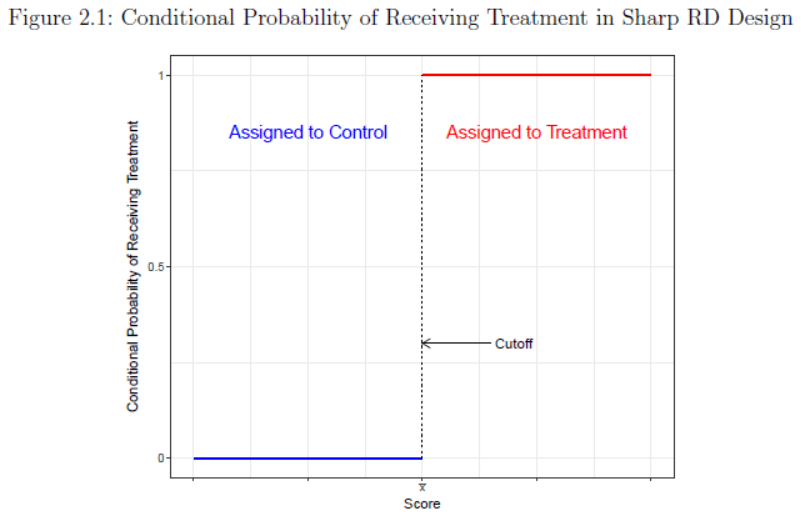
\includegraphics{"images/sharpRD.png"}
\end{frame}

\begin{frame}{The Set Up}
\protect\hypertarget{the-set-up-1}{}
The ``running variable'' \(R_i\) need not be randomly assigned:

\begin{itemize}
\item
  \(R_i\) is related to \(Y_i\)
\item
  absent treatment, this relationship is smooth (\(Y_i\) does not jump
  discontinuously as \(R_i\) changes).
\end{itemize}

\(\Rightarrow\) any discontinuous change in \(Y_i\) as \(R_i\) crosses
\(c\) can thus be interpreted as a causal effect of \(D_i\).
\end{frame}

\begin{frame}{Where to find RD setups?}
\protect\hypertarget{where-to-find-rd-setups}{}
Often from administrative situations in which units are assigned a
program, treatment or award based on a numerical index being above or
below a certain threshold.
\end{frame}

\begin{frame}{Where to find RD setups?}
\protect\hypertarget{where-to-find-rd-setups-1}{}
Examples:

\begin{itemize}
\item
  A politician may be elected if and only if the differential between
  the vote share that she receives and the vote share that her opponent
  receives exceeds 0.
\item
  A student may be assigned to summer school if and only if his
  performance on a combination of tests falls below a certain threshold.
\item
  A toxic waste site may receive cleanup funds if and only if it's
  hazard rating falls above a certain level.
\end{itemize}
\end{frame}

\begin{frame}{Why does RD work?}
\protect\hypertarget{why-does-rd-work}{}
The idea:

\begin{itemize}
\item
  Units whose indices \(R\) lie directly below the threshold \(c\) are
  considered to be comparable to individuals or units whose indices
  \(R\) lie directly above the threshold \(c\).
\item
  We can estimate the treatment effect by taking a difference in mean
  outcomes for units directly above the threshold and units directly
  below the threshold.
\end{itemize}
\end{frame}

\begin{frame}{Key RD Assumption:}
\protect\hypertarget{key-rd-assumption}{}
\textbf{The continuity assumption:}

\textbf{$E[Y_i(0)|R_i=r]$ and $E[Y_i(1)|R_i=r]$ are continuous in $r$.}

\bigskip

(Absent treatment, there would be no discontinuity in outcomes.)
\end{frame}

\begin{frame}{RD designs: The continuity assumption}
\protect\hypertarget{rd-designs-the-continuity-assumption}{}
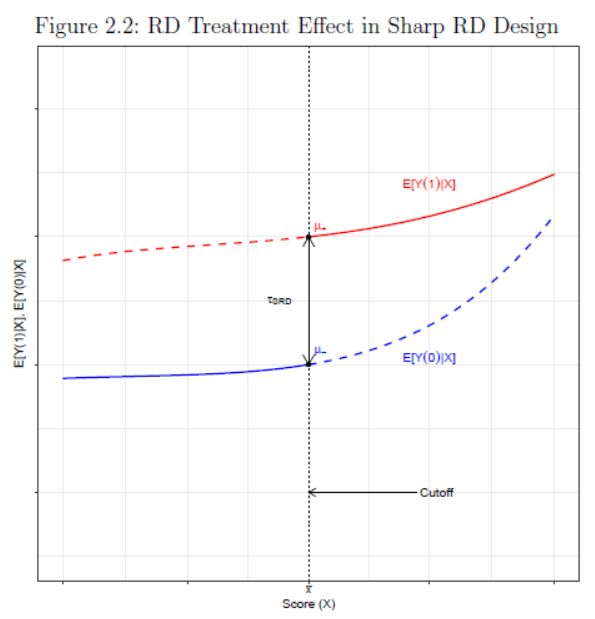
\includegraphics[width=0.75\textwidth,height=\textheight]{"images/sharpRD2.png"}
\end{frame}

\begin{frame}{RD Types}
\protect\hypertarget{rd-types}{}
RD designs come in two flavors:

\begin{itemize}
\tightlist
\item
  Sharp:

  \begin{itemize}
  \tightlist
  \item
    the probability that \(D=1\) changes from 0 to 1 as the running
    variable crosses \(c\).
  \item
    no one with \(R<c\) gets treated and everyone with \(R\geq c\) gets
    treated (or vice versa)
  \end{itemize}
\item
  Fuzzy:

  \begin{itemize}
  \tightlist
  \item
    the probability of treatment changes by some nonzero amount as the
    running variable crosses the threshold \(c\),
  \item
    the change in probability is less than 100 percentage points
    \(\Rightarrow D_i\) is no longer a deterministic function of
    \(R_i\).
  \end{itemize}
\end{itemize}

I start by discussing the general elements common to all RD designs. I
will then cover each of these specifically.
\end{frame}

\begin{frame}{RD Graphs}
\protect\hypertarget{rd-graphs}{}
Key to a good RD project is the graphical analysis (statistical results
really take a back seat).

A discontinuous change in treatment and outcomes (if \(\tau\neq 0\))
should be visible as \(R_i\) crosses the threshold \(c\).

Failure to show visually perceptible breaks at \(c\) challenges the
credibility of the approach (regardless of the regression results).

A break that is visually perceptible will almost surely be statistically
significant.
\end{frame}

\begin{frame}{RD Graphs}
\protect\hypertarget{rd-graphs-1}{}
A simple scatterplot of your data is unlikely to reveal the patterns you
wish to illustrate.

The key RD graphs are histogram-type plot that presents the average
value of:

\begin{itemize}
\item
  treatment status
\item
  the outcome
\item
  covariates
\item
  the density of the running variable
\end{itemize}

at evenly spaced values of the running variable.
\end{frame}

\begin{frame}{RD Graphs}
\protect\hypertarget{rd-graphs-2}{}
Gernerating these plots requires choosing two key parameters:

\begin{itemize}
\item
  the binwidth, \(h\),
\item
  the number of bins shown to the left and right of the threshold value,
  \(K_0\) and \(K_1\).
\end{itemize}

Once these choices are made, construct:

\begin{itemize}
\item
  \(K_0\) evenly spaced bins of width \(h\) below the threshold value
\item
  \(K_1\) evenly spaced bins of width \(h\) above the threshold value
\item
  (avoid having any bin crossing the threshold value \(c\)).
\end{itemize}
\end{frame}

\begin{frame}{RD Treatment status graph}
\protect\hypertarget{rd-treatment-status-graph}{}
RD papers often include a graph that plots treatment by the running
variable.

We expect to see a visually perceptible discontinuity in the probability
of treatment as \(R\) crosses the threshold.

After constructing the bins described above, calculate \(\bar{D}_k\),
the average treatment level in the bin

\[
\bar{D}_k=\frac{1}{N_k}\sum_{i=1}^ND_i*\mathbf{1}(b_k<R_i\leq b_{k+1}).
\]

Plot these values against the midpoint of each of the bins.
\end{frame}

\begin{frame}{Outcome Graphs}
\protect\hypertarget{outcome-graphs}{}
The main course of an RD paper is a plot of the outcome by the running
variable.

If \(\tau\neq0\), we expect to see a discontinuity here too.

Plotting this graph requires calculating, \(\bar{Y}_k\), the average
outcome in each bin

\[
\bar{Y}_k=\frac{1}{N_k}\sum_{i=1}^NY_i*\mathbf{1}(b_k<R_i\leq b_{k+1})
\]

and plotting these values against the midpoint of each of the bins.
\end{frame}

\begin{frame}{Outcome Graphs}
\protect\hypertarget{outcome-graphs-1}{}
A visual break at \(c\)

\begin{itemize}
\item
  \(\Rightarrow\) crossing \(c\) has a significant effect on the
  outcome,
\item
  \(\Rightarrow\) the treatment has a significant effect on the outcome.
  This graph is the equivalent of the reduced form in an IV analysis.
\end{itemize}
\end{frame}

\begin{frame}{Outcome Graphs: Robustness}
\protect\hypertarget{outcome-graphs-robustness}{}
You should also look for other discontinuities of similar (or greater)
magnitude at other values of \(R\).

If there discontinuities for no clear reason, the research design is
called into question - effectively we have detected a violation of
Assumption 1 (smoothness in expected potential outcomes).
\end{frame}

\begin{frame}{Robustness Graphs: Covariates}
\protect\hypertarget{robustness-graphs-covariates}{}
It is common to plot covariates that may be related to the outcome but
should not be affected by the treatment.

As above, we calculate \(\bar{X}_k\) where \[
\bar{X}_k=\frac{1}{N_k}\sum_{i=1}^NX_i*\mathbf{1}(b_k<R_i\leq b_{k+1})
\] is plotted against the midpoint of each bin.

If the research design is valid there should not be any discontinuity in
\(\bar{X}_k\) as the running variable crosses the threshold \(c\).

This is equivalent to a balance check across the threshold- you are
checking that the treated and un-treated groups are similar.
\end{frame}

\begin{frame}{Robustness Graphs: Density of the Running Variable}
\protect\hypertarget{robustness-graphs-density-of-the-running-variable}{}
It is also common to plot the density of the running variable.

For each bin, you calculate \[
N_k=\sum_{i=1}^N\mathbf{1}(b_k<R_i\leq b_{k+1})
\] and plot these against the midpoint of the bin.

A concern in RD is that individuals may ``game'' the assignment rule:
they manipulate their \(R_i\) to place themselves just above (below)
\(c\).

This sorting would create selection bias and bias our estimate of
\(\tau\).

If units are manipulating \(R_i\) around \(c\), we will see a
discontinuity in the distribution of \(R_i\) as it crosses \(c\).

If the distribution of \(R_i\) is smooth as it crosses \(c\), then it's
unlikely that individuals are gaming the assignment mechanism.
\end{frame}

\begin{frame}{Robustness Graphs: Density of the Running Variable}
\protect\hypertarget{robustness-graphs-density-of-the-running-variable-1}{}
Example:

\begin{itemize}
\item
  consider a scholarship if test scores fall above a certain threshold
  \(c\). Shrewd students could retake the test many times until they
  pass the threshold.
\item
  If a researcher uses an individuals maximum test score as the running
  variable, motivated individuals who retake the test many times are
  more likely to fall just above the threshold, then just below it.
\item
  this group of observations is selected and no longer directly
  comparable to the observations that fall directly below the threshold.
\end{itemize}
\end{frame}

\begin{frame}{RD Estimation}
\protect\hypertarget{rd-estimation}{}
RD estimations can be done quite easily in a regression framework.

There are a couple things to keep in mind when it comes to RD estimation
strategies:

\begin{itemize}
\item
  the choice of functional form
\item
  the choice of bandwidth.
\end{itemize}
\end{frame}

\begin{frame}{RD Estimation: Functional form}
\protect\hypertarget{rd-estimation-functional-form}{}
To identify the treatment effect, you need a good model of the
underlying relationship between the running variable and the outcome.
\end{frame}

\begin{frame}{RD Estimation: Functional form}
\protect\hypertarget{rd-estimation-functional-form-1}{}
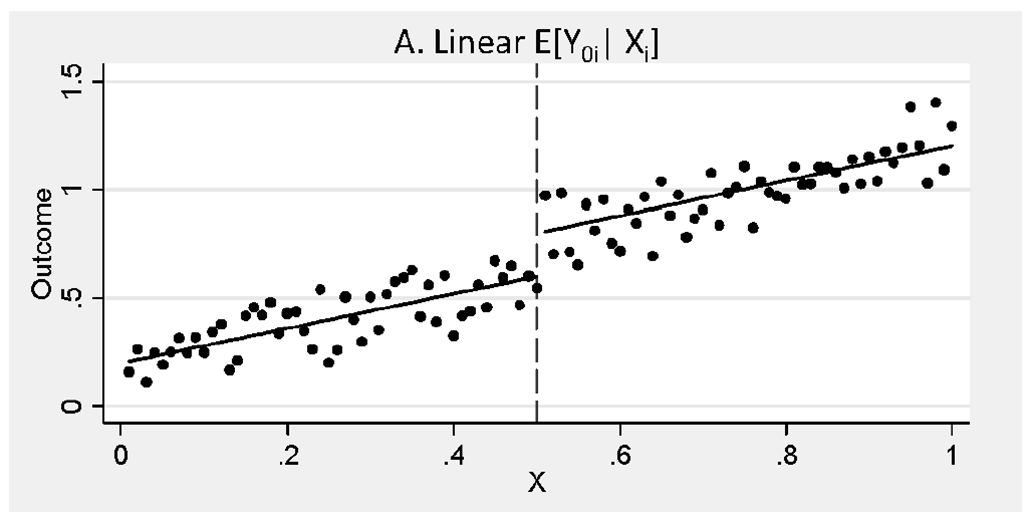
\includegraphics[width=0.75\textwidth,height=\textheight]{"images/rdlinear.png"}

Easy if the underlying relatonship is linear:

\begin{itemize}
\item
  a linear regression fits the data well
\item
  the treatment effect is the ``jump'' between the intercepts at the
  threshold value.
\end{itemize}
\end{frame}

\begin{frame}{RD Estimation: Functional form}
\protect\hypertarget{rd-estimation-functional-form-2}{}
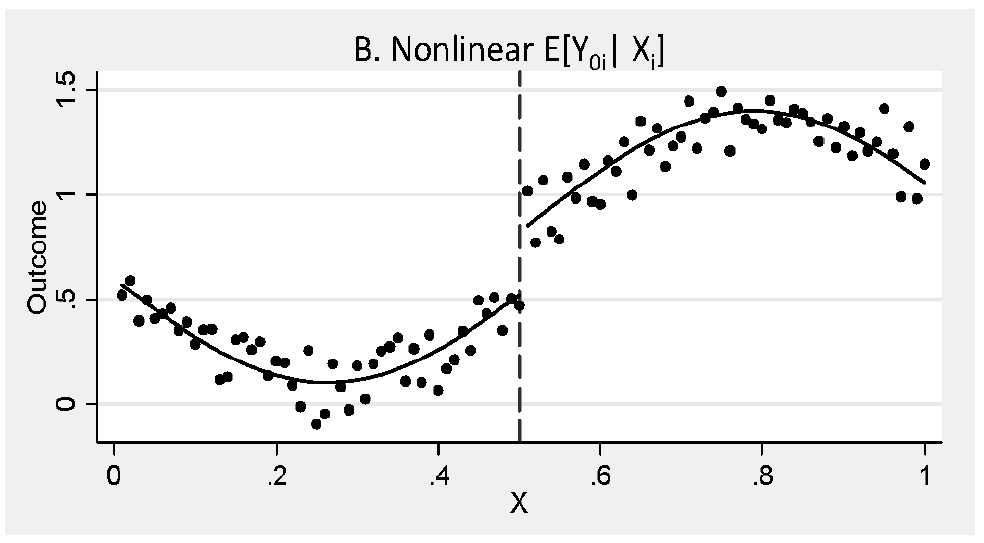
\includegraphics[width=0.75\textwidth,height=\textheight]{"images/RDnonlin.png"}

If not linear, need higher order polynomial terms.

\textbf{What if I fit a linear function?}
\end{frame}

\begin{frame}{RD Estimation: Functional form}
\protect\hypertarget{rd-estimation-functional-form-3}{}
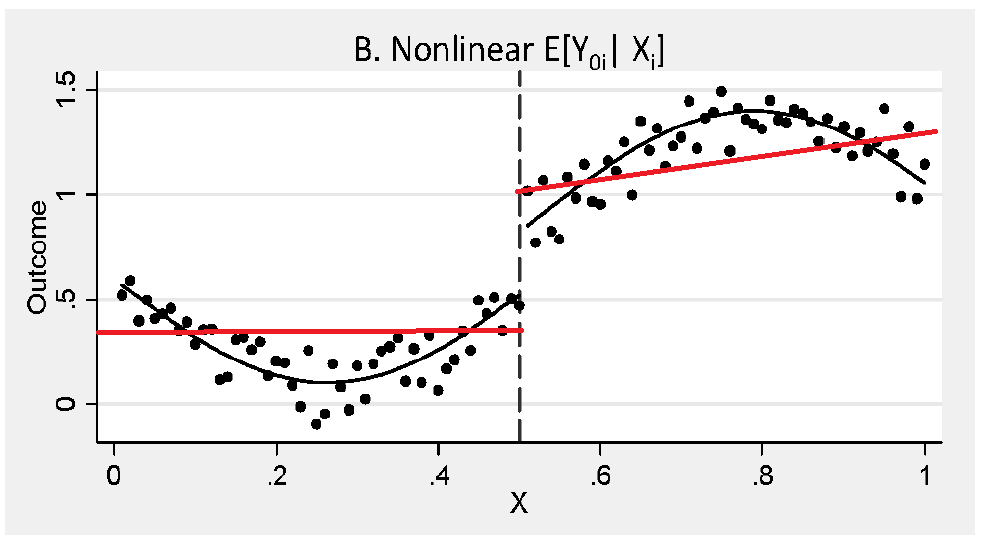
\includegraphics[width=0.75\textwidth,height=\textheight]{"images/RDnonlinlin.png"}

If not linear, need higher order polynomial terms.

\textbf{What if I fit a linear function?}

If we do not fit the data correctly, the ``jump'' at the the threshold
will not correctly estimate the treatment effect.
\end{frame}

\begin{frame}{RD Estimation: Functional form}
\protect\hypertarget{rd-estimation-functional-form-4}{}
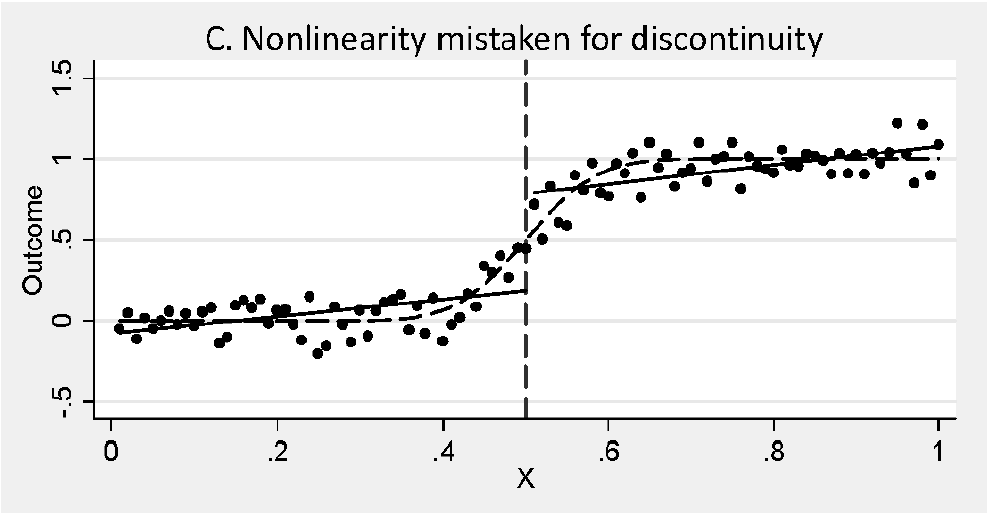
\includegraphics[width=0.75\textwidth,height=\textheight]{"images/RDmistake.png"}

There is no discontinuity at the threshold.

If I force a linear regression to this data I will detect a
discontinuity: I find a treatment effect where there is none.
\end{frame}

\begin{frame}{RD Estimation: Robustness to functional form}
\protect\hypertarget{rd-estimation-robustness-to-functional-form}{}
Good graphs are important: they will alert you to these problems.

Run specifications with higher order polynomials and check that your
estimated treatment effect is not sensitive to their inclusion (or
exclusion).
\end{frame}

\begin{frame}{RD Estimation: Choosing the bandwidth}
\protect\hypertarget{rd-estimation-choosing-the-bandwidth}{}
The bandwidth: how close to the threshold an observation's running
variable must be to be in the regression sample.

\textbf{What bandwidth, \(h\), should you use?}

There is an econometric literature on this.

In practice this choice is more art than science (ie fairly arbitrary).
\end{frame}

\begin{frame}{RD Estimation: Choosing the bandwidth}
\protect\hypertarget{rd-estimation-choosing-the-bandwidth-1}{}
The choice is a tradeoff:

\begin{itemize}
\item
  With a large bandwidth, you will have a larger sample which can shrink
  your standard errors and improve the precision of your results.
\item
  Two main drawbacks to a large bandwidth:

  \begin{itemize}
  \item
    With a very large bandwith, it becomes more difficult to argue that
    observations on either side of the threshold are similar.
  \item
    Making sure you select the right functional form will be more
    important if you are working with a wide bandwith. Example: see
    figure C.
  \end{itemize}
\item
  Good practice: check that results are not sensitive to the choice of
  bandwidth.
\end{itemize}
\end{frame}

\begin{frame}{RD Estimation}
\protect\hypertarget{rd-estimation-1}{}
The specifics of the estimation will depend on whether we are dealing
with a sharp or fuzzy RD.
\end{frame}

\hypertarget{sharp-rd}{%
\section{Sharp RD}\label{sharp-rd}}

\begin{frame}{Sharp RD Set up:}
\protect\hypertarget{sharp-rd-set-up}{}
The probability that \(D=1\) changes from 0 to 1 as the running variable
crosses \(c\).

\begin{itemize}
\item
  no one with \(R_i<c\) gets treated
\item
  everyone with \(R_i\geq c\) gets treated
\item
  \(\Rightarrow D_i\) is a deterministic function of \(R_i: D_i=1\) if
  \((R_i\geq c)\).
\item
  (or vice versa)
\end{itemize}
\end{frame}

\begin{frame}{Sharp RD Set up:}
\protect\hypertarget{sharp-rd-set-up-1}{}
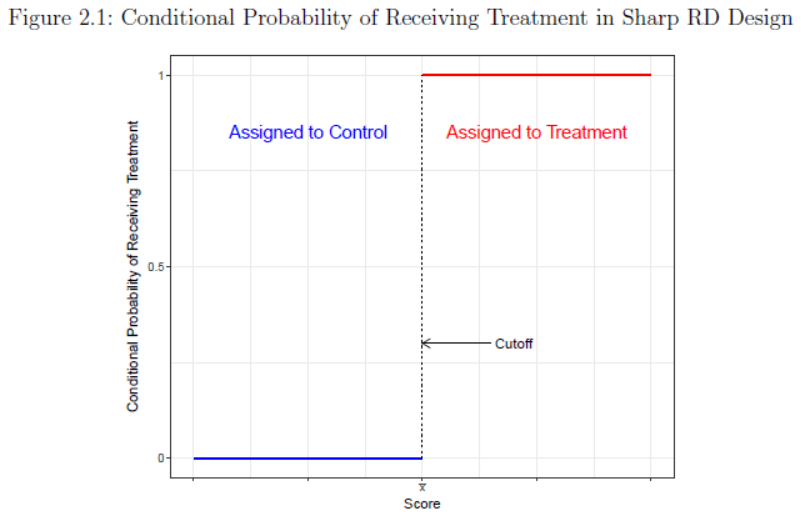
\includegraphics{"images/sharpRD.png"}
\end{frame}

\begin{frame}{Sharp RD Set up:}
\protect\hypertarget{sharp-rd-set-up-2}{}
To estimate the causal effect of \(D_i\) on some outcome \(Y_i\), we
simply take the difference in mean outcome on either side of \(c\):

\footnotesize

\[
\lim\limits_{r \rightarrow c}E[Y_i|R_i=r]-\lim\limits_{r \leftarrow c}E[Y_i|R_i=r]=\lim\limits_{r \rightarrow c}E[Y_i(1)|R_i=r]-\lim\limits_{r \leftarrow c}E[Y_i(0)|R_i=r]
\]

\normalsize

This estimates \(\tau_{SRD}\), the causal effect for individuals with
\(R_i=c\):

\[
\tau_{SRD}=E[Y_i(1)-Y_i(0)|R_i=c]
\]
\end{frame}

\begin{frame}{Sharp RD Assumption:}
\protect\hypertarget{sharp-rd-assumption}{}
If the continuity assumption holds:

\[
\tau_{SRD}=\lim\limits_{r \rightarrow c}E[Y_i|R_i=r]-\lim\limits_{r \leftarrow c}E[Y_i|R_i=r]
\]

\bigskip

We can estimate \(\tau_{SRD}\) as the difference between the two
regression functions estimated in the \textbf{neighborhood} of \(c\).
\end{frame}

\begin{frame}{Sharp RD designs:}
\protect\hypertarget{sharp-rd-designs}{}
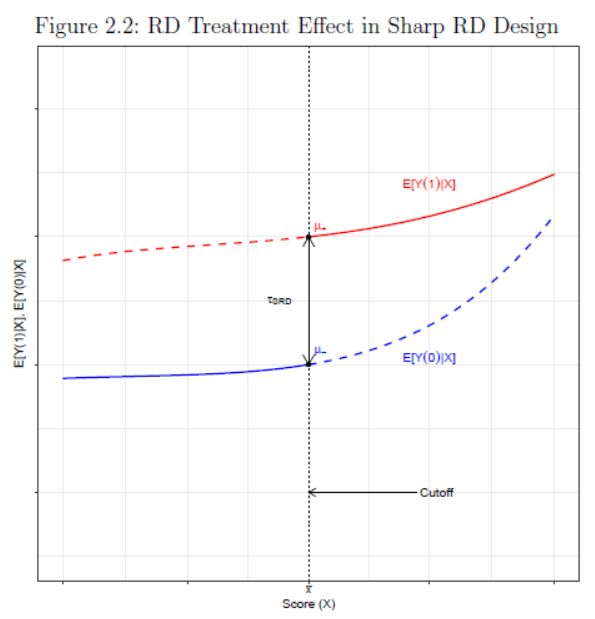
\includegraphics[width=0.75\textwidth,height=\textheight]{"images/sharpRD2.png"}
\end{frame}

\begin{frame}{Sharp RD Simulation}
\protect\hypertarget{sharp-rd-simulation}{}
You are the superintendent of a large school district.

Last year you made participation in small reading groups
\textbf{mandatory} for all students whose 3rd grade reading score was 75
points or less.

Your data includes the 3rd and 4th grade reading scores for all 5000
students in your school district.

\textbf{How did these reading groups affected student performance on
their 4th grade reading tests?}
\end{frame}

\begin{frame}[fragile]{Sharp RD Simulation}
\protect\hypertarget{sharp-rd-simulation-1}{}
\small

\begin{Shaded}
\begin{Highlighting}[]
\FunctionTok{set.seed}\NormalTok{(}\DecValTok{7000}\NormalTok{)}

\NormalTok{sharp}\OtherTok{\textless{}{-}}\FunctionTok{rnorm}\NormalTok{(}\DecValTok{5000}\NormalTok{, }\AttributeTok{mean=}\DecValTok{80}\NormalTok{, }\AttributeTok{sd=}\DecValTok{5}\NormalTok{)}
\NormalTok{sharp}\OtherTok{\textless{}{-}}\FunctionTok{as.data.frame}\NormalTok{(sharp)}

\FunctionTok{names}\NormalTok{(sharp)}\OtherTok{\textless{}{-}}\FunctionTok{c}\NormalTok{(}\StringTok{"read3"}\NormalTok{)}
\NormalTok{sharp}\SpecialCharTok{$}\NormalTok{error}\OtherTok{\textless{}{-}}\FunctionTok{rnorm}\NormalTok{(}\DecValTok{5000}\NormalTok{, }\AttributeTok{mean=}\DecValTok{0}\NormalTok{, }\AttributeTok{sd=}\DecValTok{5}\NormalTok{)}
\NormalTok{sharp}\SpecialCharTok{$}\NormalTok{pe3}\OtherTok{\textless{}{-}}\FunctionTok{rnorm}\NormalTok{(}\DecValTok{5000}\NormalTok{, }\AttributeTok{mean=}\DecValTok{90}\NormalTok{, }\AttributeTok{sd=}\DecValTok{4}\NormalTok{)}
\NormalTok{sharp}\SpecialCharTok{$}\NormalTok{height}\OtherTok{\textless{}{-}}\FunctionTok{rnorm}\NormalTok{(}\DecValTok{5000}\NormalTok{, }\AttributeTok{mean=}\DecValTok{130}\NormalTok{, }\AttributeTok{sd=}\DecValTok{15}\NormalTok{)}
\end{Highlighting}
\end{Shaded}
\end{frame}

\begin{frame}[fragile]{Sharp RD Simulation}
\protect\hypertarget{sharp-rd-simulation-2}{}
\small

\begin{Shaded}
\begin{Highlighting}[]
\NormalTok{sharp}\SpecialCharTok{$}\NormalTok{treated}\OtherTok{\textless{}{-}}\DecValTok{0}
\NormalTok{sharp}\SpecialCharTok{$}\NormalTok{treated[sharp}\SpecialCharTok{$}\NormalTok{read3}\SpecialCharTok{\textless{}=}\DecValTok{75}\NormalTok{]}\OtherTok{\textless{}{-}}\DecValTok{1}

\NormalTok{tau}\OtherTok{=}\DecValTok{10}
\CommentTok{\#the DGP}
\NormalTok{sharp}\SpecialCharTok{$}\NormalTok{read4}\OtherTok{\textless{}{-}}\NormalTok{(}\SpecialCharTok{{-}}\DecValTok{6}\NormalTok{)}\SpecialCharTok{+}\FloatTok{0.8}\SpecialCharTok{*}\NormalTok{sharp}\SpecialCharTok{$}\NormalTok{read3}\SpecialCharTok{+}\NormalTok{tau}\SpecialCharTok{*}\NormalTok{sharp}\SpecialCharTok{$}\NormalTok{treated}\SpecialCharTok{+}\NormalTok{sharp}\SpecialCharTok{$}\NormalTok{error}

\CommentTok{\#selecting observations that fall in our bandwidth}
\NormalTok{sharp}\OtherTok{\textless{}{-}}\NormalTok{sharp[sharp}\SpecialCharTok{$}\NormalTok{read3}\SpecialCharTok{\textless{}}\DecValTok{78} \SpecialCharTok{\&}\NormalTok{ sharp}\SpecialCharTok{$}\NormalTok{read3}\SpecialCharTok{\textgreater{}}\DecValTok{72}\NormalTok{,]}
\end{Highlighting}
\end{Shaded}
\end{frame}

\begin{frame}{Sharp RD: Treatment status graph}
\protect\hypertarget{sharp-rd-treatment-status-graph}{}
\begin{itemize}
\item
  Step 1: construct the histogram bins
\item
  Step 2: calculate \(\bar{D}_k\), the average treatment level in the
  bin
\end{itemize}

\[
\bar{D}_k=\frac{1}{N_k}\sum_{i=1}^ND_i*\mathbf{1}(b_k<R_i\leq b_{k+1}).
\]

In a sharp RD, \(\bar{D}_k\) should be either 0 or 1.
\end{frame}

\begin{frame}[fragile]{Sharp RD: Treatment status graph Simulation}
\protect\hypertarget{sharp-rd-treatment-status-graph-simulation}{}
\tiny

\begin{Shaded}
\begin{Highlighting}[]
\CommentTok{\#I will break up the data into 60 bins (30 above and 30 below the threshold)}
\NormalTok{cuts}\OtherTok{\textless{}{-}}\FunctionTok{c}\NormalTok{(}\DecValTok{72}\NormalTok{,}\FloatTok{72.1}\NormalTok{,}\FloatTok{72.2}\NormalTok{,}\FloatTok{72.3}\NormalTok{,}\FloatTok{72.4}\NormalTok{,}\FloatTok{72.5}\NormalTok{,}\FloatTok{72.6}\NormalTok{,}\FloatTok{72.7}\NormalTok{,}\FloatTok{72.8}\NormalTok{,}\FloatTok{72.9}\NormalTok{,}\DecValTok{73}\NormalTok{,}
        \FloatTok{73.1}\NormalTok{,}\FloatTok{73.2}\NormalTok{,}\FloatTok{73.3}\NormalTok{,}\FloatTok{73.4}\NormalTok{,}\FloatTok{73.5}\NormalTok{,}\FloatTok{73.6}\NormalTok{,}\FloatTok{73.7}\NormalTok{,}\FloatTok{73.8}\NormalTok{,}\FloatTok{73.9}\NormalTok{,}\DecValTok{74}\NormalTok{,}
        \FloatTok{74.1}\NormalTok{,}\FloatTok{74.2}\NormalTok{,}\FloatTok{74.3}\NormalTok{,}\FloatTok{74.4}\NormalTok{,}\FloatTok{74.5}\NormalTok{,}\FloatTok{74.6}\NormalTok{,}\FloatTok{74.7}\NormalTok{,}\FloatTok{74.8}\NormalTok{,}\FloatTok{74.9}\NormalTok{,}\DecValTok{75}\NormalTok{,}
        \FloatTok{75.1}\NormalTok{,}\FloatTok{75.2}\NormalTok{,}\FloatTok{75.3}\NormalTok{,}\FloatTok{75.4}\NormalTok{,}\FloatTok{75.5}\NormalTok{,}\FloatTok{75.6}\NormalTok{,}\FloatTok{75.7}\NormalTok{,}\FloatTok{75.8}\NormalTok{,}\FloatTok{75.9}\NormalTok{,}\DecValTok{76}\NormalTok{,}
        \FloatTok{76.1}\NormalTok{,}\FloatTok{76.2}\NormalTok{,}\FloatTok{76.3}\NormalTok{,}\FloatTok{76.4}\NormalTok{,}\FloatTok{76.5}\NormalTok{,}\FloatTok{76.6}\NormalTok{,}\FloatTok{76.7}\NormalTok{,}\FloatTok{76.8}\NormalTok{,}\FloatTok{76.9}\NormalTok{,}\DecValTok{77}\NormalTok{,}
        \FloatTok{77.1}\NormalTok{,}\FloatTok{77.2}\NormalTok{,}\FloatTok{77.3}\NormalTok{,}\FloatTok{77.4}\NormalTok{,}\FloatTok{77.5}\NormalTok{,}\FloatTok{77.6}\NormalTok{,}\FloatTok{77.7}\NormalTok{,}\FloatTok{77.8}\NormalTok{,}\FloatTok{77.9}\NormalTok{,}\DecValTok{78}\NormalTok{)}
\NormalTok{midpoints}\OtherTok{\textless{}{-}}\NormalTok{cuts[}\DecValTok{2}\SpecialCharTok{:}\DecValTok{61}\NormalTok{]}\SpecialCharTok{{-}}\FloatTok{0.05}

\NormalTok{sharp}\SpecialCharTok{$}\NormalTok{bins }\OtherTok{\textless{}{-}} \FunctionTok{cut}\NormalTok{(sharp}\SpecialCharTok{$}\NormalTok{read3, }
                  \AttributeTok{breaks=}\NormalTok{cuts, }
                  \AttributeTok{include.lowest=}\ConstantTok{TRUE}\NormalTok{, }
                  \AttributeTok{right=}\ConstantTok{FALSE}\NormalTok{, }
                  \AttributeTok{labels=}\NormalTok{midpoints)}


\NormalTok{sharp\_mean}\OtherTok{\textless{}{-}}\NormalTok{sharp }\SpecialCharTok{\%\textgreater{}\%}
    \FunctionTok{group\_by}\NormalTok{(bins) }\SpecialCharTok{\%\textgreater{}\%}
\NormalTok{    dplyr}\SpecialCharTok{::}\FunctionTok{summarize}\NormalTok{(}\AttributeTok{outbinmean =} \FunctionTok{mean}\NormalTok{(read4, }\AttributeTok{na.rm=}\ConstantTok{TRUE}\NormalTok{),}
                     \AttributeTok{treatbinmean=}\FunctionTok{mean}\NormalTok{(treated, }\AttributeTok{na.rm=}\ConstantTok{TRUE}\NormalTok{), }
                     \AttributeTok{pebinmean=}\FunctionTok{mean}\NormalTok{(pe3, }\AttributeTok{na.rm=}\ConstantTok{TRUE}\NormalTok{),}
                     \AttributeTok{heightbinmean=}\FunctionTok{mean}\NormalTok{(height, }\AttributeTok{na.rm=}\ConstantTok{TRUE}\NormalTok{), }\AttributeTok{numb=}\FunctionTok{n}\NormalTok{())}

\NormalTok{sharp\_mean}\SpecialCharTok{$}\NormalTok{bins}\OtherTok{\textless{}{-}}\FunctionTok{as.numeric}\NormalTok{(}\FunctionTok{as.character}\NormalTok{(sharp\_mean}\SpecialCharTok{$}\NormalTok{bins))}

\NormalTok{plot1shp}\OtherTok{\textless{}{-}}\FunctionTok{ggplot}\NormalTok{(sharp\_mean, }\FunctionTok{aes}\NormalTok{(}\AttributeTok{x=}\NormalTok{bins, }\AttributeTok{y=}\NormalTok{treatbinmean))}\SpecialCharTok{+} 
         \FunctionTok{geom\_point}\NormalTok{()}\SpecialCharTok{+}
         \FunctionTok{geom\_vline}\NormalTok{(}\AttributeTok{xintercept =} \DecValTok{75}\NormalTok{)}
\end{Highlighting}
\end{Shaded}
\end{frame}

\begin{frame}[fragile]{Sharp RD: Treatment status graph Simulation}
\protect\hypertarget{sharp-rd-treatment-status-graph-simulation-1}{}
\begin{Shaded}
\begin{Highlighting}[]
\NormalTok{plot1shp}
\end{Highlighting}
\end{Shaded}

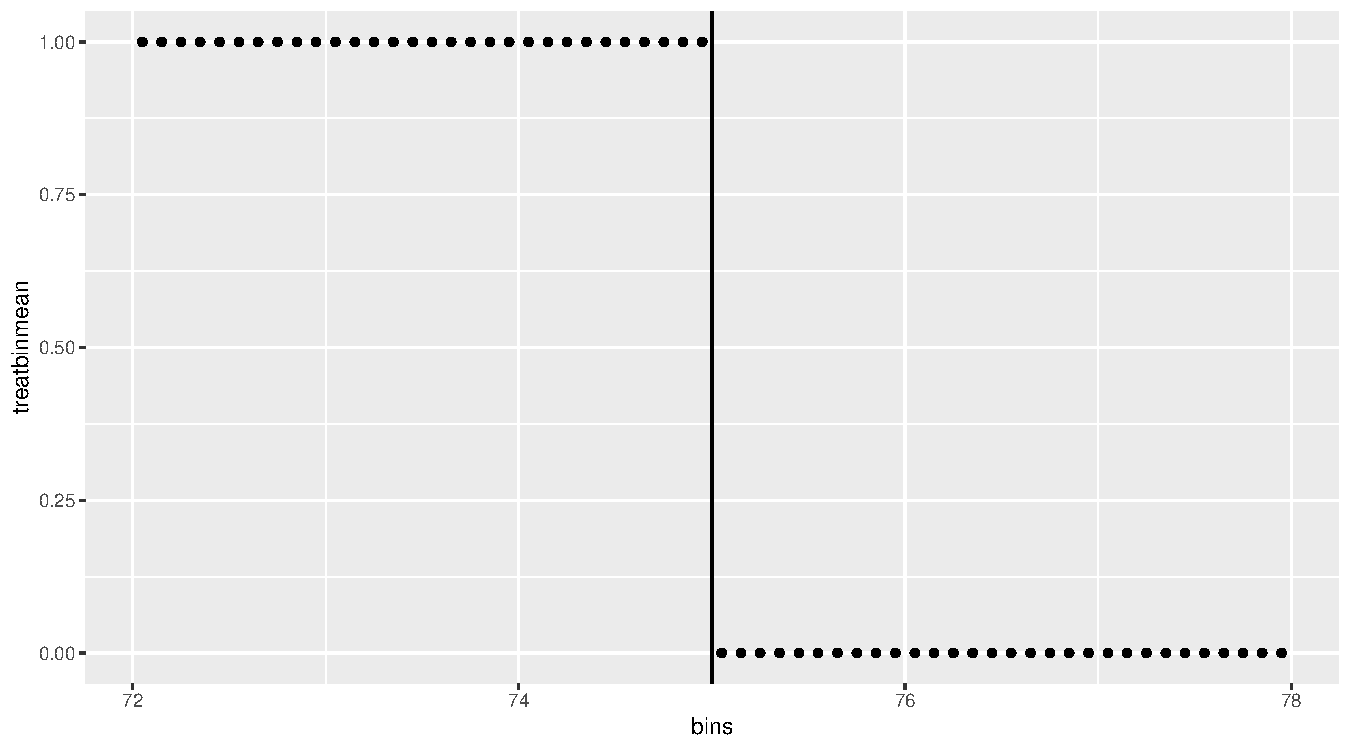
\includegraphics{Slides9_RD_files/figure-beamer/sharp2b-1.pdf}
\end{frame}

\begin{frame}[fragile]{Outcome Graphs: Sharp}
\protect\hypertarget{outcome-graphs-sharp}{}
In the earlier chunk, we calculated, \(\bar{Y}_k\), the average outcome
in each bin

\[
\bar{Y}_k=\frac{1}{N_k}\sum_{i=1}^NY_i*\mathbf{1}(b_k<R_i\leq b_{k+1})
\] \tiny

\begin{Shaded}
\begin{Highlighting}[]
\NormalTok{plot2shp}\OtherTok{\textless{}{-}}\FunctionTok{ggplot}\NormalTok{(sharp\_mean, }\FunctionTok{aes}\NormalTok{(}\AttributeTok{x=}\NormalTok{bins, }\AttributeTok{y=}\NormalTok{outbinmean))}\SpecialCharTok{+} 
         \FunctionTok{geom\_point}\NormalTok{()}\SpecialCharTok{+}
         \FunctionTok{geom\_vline}\NormalTok{(}\AttributeTok{xintercept =} \DecValTok{75}\NormalTok{)}
\end{Highlighting}
\end{Shaded}
\end{frame}

\begin{frame}{Outcome Graphs: Sharp}
\protect\hypertarget{outcome-graphs-sharp-1}{}
\tiny

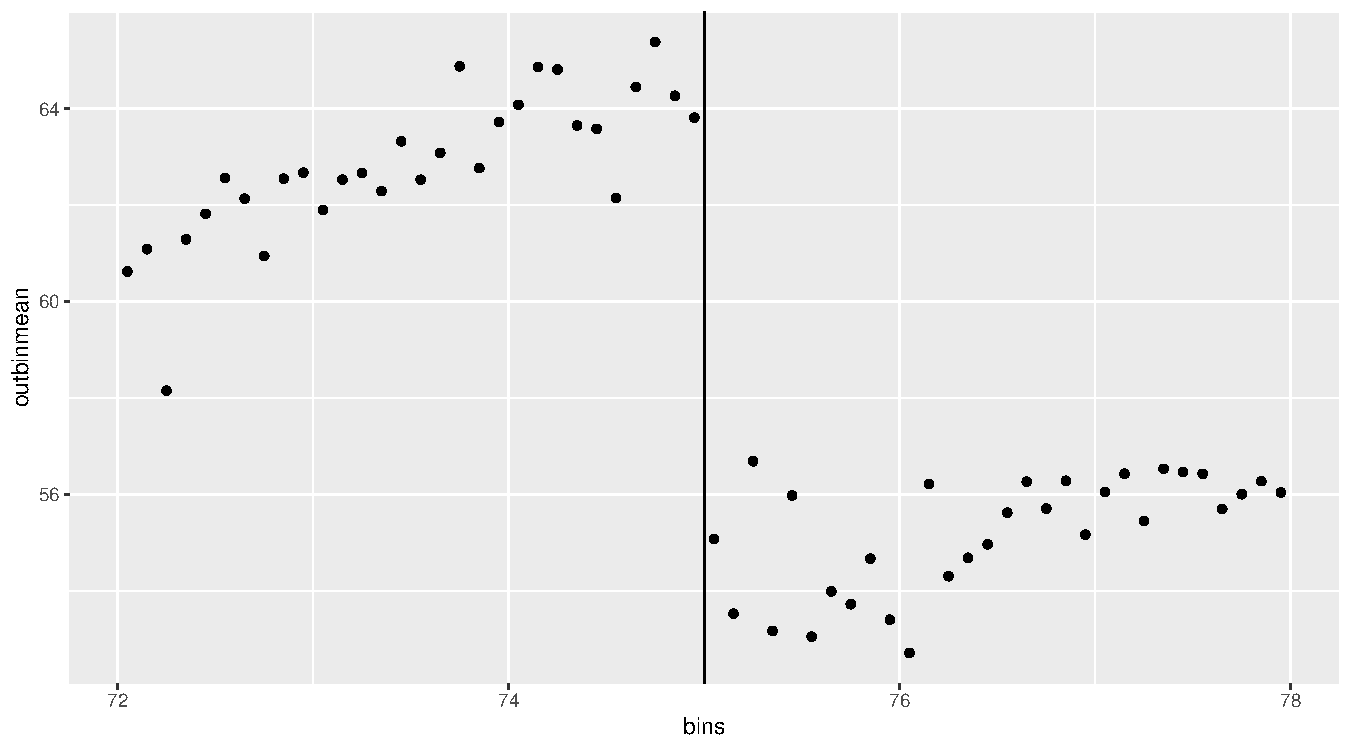
\includegraphics{Slides9_RD_files/figure-beamer/sharp3b-1.pdf}
\end{frame}

\begin{frame}[fragile]{Robustness Graphs: Covariates sharp}
\protect\hypertarget{robustness-graphs-covariates-sharp}{}
In the earlier chunk, we calculated \(\bar{X}_k\) where \[
\bar{X}_k=\frac{1}{N_k}\sum_{i=1}^NX_i*\mathbf{1}(b_k<R_i\leq b_{k+1})
\]

\tiny

\begin{Shaded}
\begin{Highlighting}[]
\NormalTok{plot3shp}\OtherTok{\textless{}{-}}\FunctionTok{ggplot}\NormalTok{(sharp\_mean, }\FunctionTok{aes}\NormalTok{(}\AttributeTok{x=}\NormalTok{bins, }\AttributeTok{y=}\NormalTok{pebinmean))}\SpecialCharTok{+} 
         \FunctionTok{geom\_point}\NormalTok{()}\SpecialCharTok{+}
         \FunctionTok{geom\_vline}\NormalTok{(}\AttributeTok{xintercept =} \DecValTok{75}\NormalTok{)}
\end{Highlighting}
\end{Shaded}
\end{frame}

\begin{frame}[fragile]{Robustness Graphs: Covariates sharp}
\protect\hypertarget{robustness-graphs-covariates-sharp-1}{}
\begin{Shaded}
\begin{Highlighting}[]
\NormalTok{plot3shp}
\end{Highlighting}
\end{Shaded}

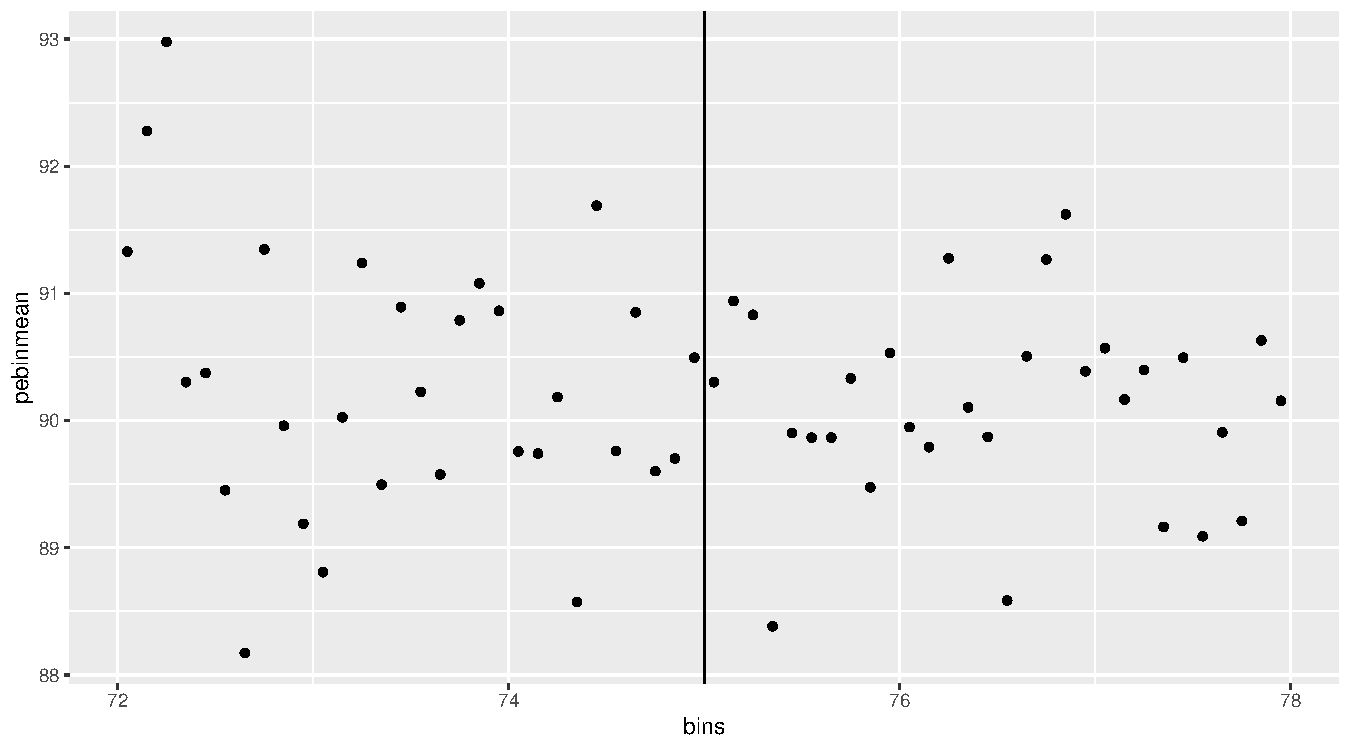
\includegraphics{Slides9_RD_files/figure-beamer/sharp4d-1.pdf}
\end{frame}

\begin{frame}[fragile]{Robustness Graphs: Covariates sharp}
\protect\hypertarget{robustness-graphs-covariates-sharp-2}{}
\tiny

\begin{Shaded}
\begin{Highlighting}[]
\NormalTok{plot4shp}\OtherTok{\textless{}{-}}\FunctionTok{ggplot}\NormalTok{(sharp\_mean, }\FunctionTok{aes}\NormalTok{(}\AttributeTok{x=}\NormalTok{bins, }\AttributeTok{y=}\NormalTok{heightbinmean))}\SpecialCharTok{+} 
         \FunctionTok{geom\_point}\NormalTok{()}\SpecialCharTok{+}
         \FunctionTok{geom\_vline}\NormalTok{(}\AttributeTok{xintercept =} \DecValTok{75}\NormalTok{)}
\NormalTok{plot4shp}
\end{Highlighting}
\end{Shaded}

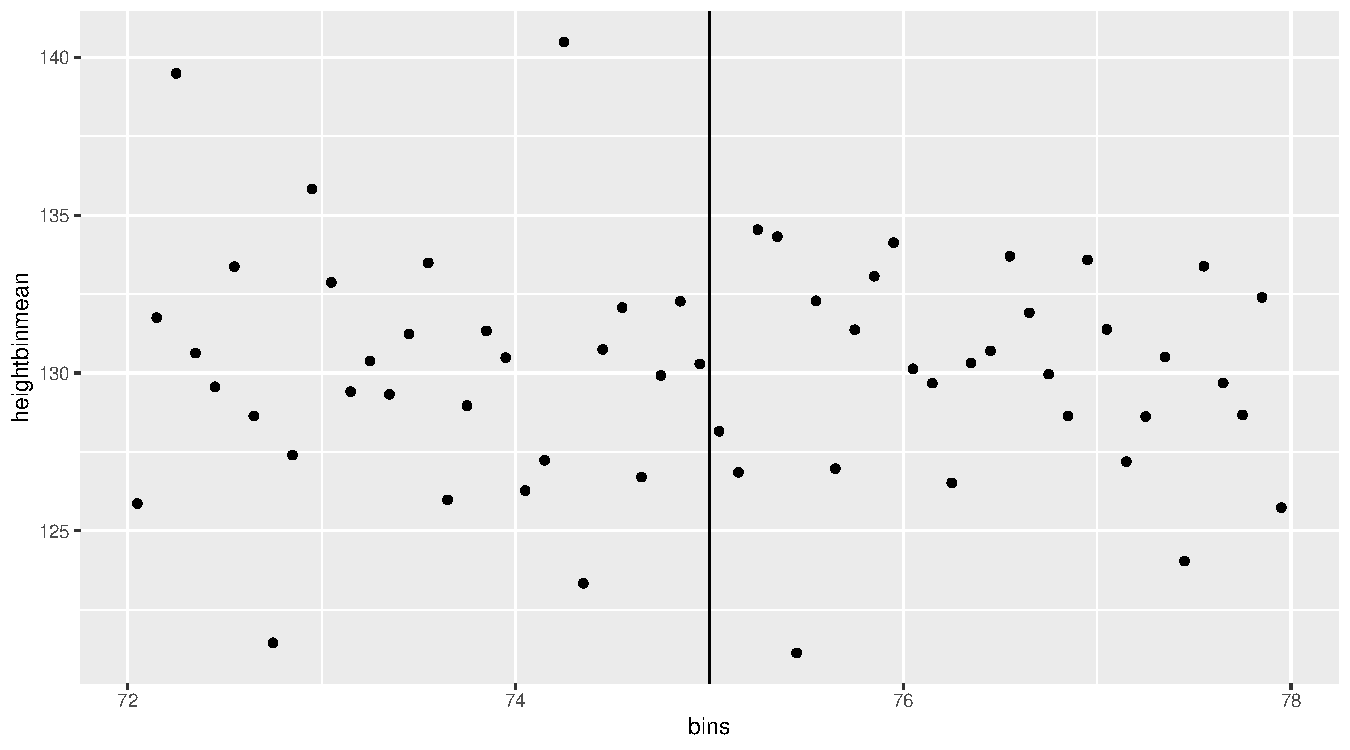
\includegraphics{Slides9_RD_files/figure-beamer/sharp4b-1.pdf}
\end{frame}

\begin{frame}[fragile]{Robustness Graphs: Density of the Running
Variable (Sharp)}
\protect\hypertarget{robustness-graphs-density-of-the-running-variable-sharp}{}
In an earlier chunk we calculated \[
N_k=\sum_{i=1}^N\mathbf{1}(b_k<R_i\leq b_{k+1})
\] \tiny

\begin{Shaded}
\begin{Highlighting}[]
\NormalTok{plot5shp}\OtherTok{\textless{}{-}}\FunctionTok{ggplot}\NormalTok{(sharp\_mean, }\FunctionTok{aes}\NormalTok{(}\AttributeTok{x=}\NormalTok{bins, }\AttributeTok{y=}\NormalTok{numb))}\SpecialCharTok{+} 
         \FunctionTok{geom\_point}\NormalTok{()}\SpecialCharTok{+}
         \FunctionTok{geom\_vline}\NormalTok{(}\AttributeTok{xintercept =} \DecValTok{75}\NormalTok{)}
\end{Highlighting}
\end{Shaded}
\end{frame}

\begin{frame}[fragile]{Robustness Graphs: Density of the Running
Variable (Sharp)}
\protect\hypertarget{robustness-graphs-density-of-the-running-variable-sharp-1}{}
\begin{Shaded}
\begin{Highlighting}[]
\NormalTok{plot5shp}
\end{Highlighting}
\end{Shaded}

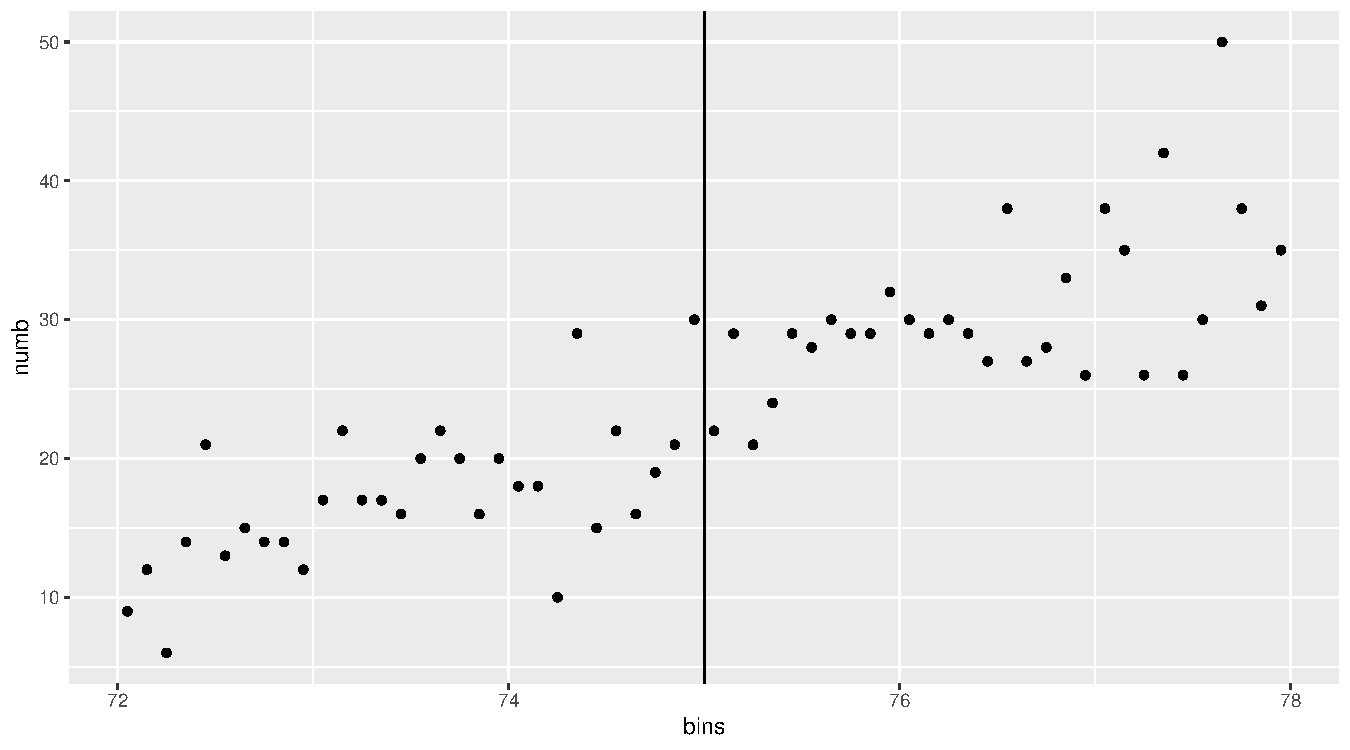
\includegraphics{Slides9_RD_files/figure-beamer/sharp5a-1.pdf}
\end{frame}

\begin{frame}{RD Estimation: Sharp}
\protect\hypertarget{rd-estimation-sharp}{}
Idea: Fit a linear regression on either side of the threshold point for
the samples with \(R_i\in (c-h,c)\) and \(R_i[c,c+h)\).

Estimate some version (you can include covariates) of the following
specification, \[
Y_i=\alpha+\tau D_i+\beta(R_i-c)+\gamma (R_i-c)*D_i+u_i \text{ for }  c-h\leq R_i< c+h. 
\]

With this estimation strategy, \(\hat{\tau}_{SRD}\) will estimate the
treatment effect for units right at the threshold.
\end{frame}

\begin{frame}[fragile]{RD Estimation: Sharp}
\protect\hypertarget{rd-estimation-sharp-1}{}
\tiny

\begin{Shaded}
\begin{Highlighting}[]
\NormalTok{sharp}\SpecialCharTok{$}\NormalTok{runminc}\OtherTok{\textless{}{-}}\NormalTok{sharp}\SpecialCharTok{$}\NormalTok{read3}\DecValTok{{-}75}
\NormalTok{shpestim}\OtherTok{\textless{}{-}}\FunctionTok{felm}\NormalTok{(read4}\SpecialCharTok{\textasciitilde{}}\NormalTok{treated}\SpecialCharTok{+}\NormalTok{runminc}\SpecialCharTok{+}\NormalTok{treated}\SpecialCharTok{*}\NormalTok{runminc, sharp)}

\FunctionTok{stargazer}\NormalTok{(shpestim, }\AttributeTok{type=}\StringTok{"latex"}\NormalTok{, }\AttributeTok{header=}\ConstantTok{FALSE}\NormalTok{)}
\end{Highlighting}
\end{Shaded}

\begin{table}[!htbp] \centering 
  \caption{} 
  \label{} 
\begin{tabular}{@{\extracolsep{5pt}}lc} 
\\[-1.8ex]\hline 
\hline \\[-1.8ex] 
 & \multicolumn{1}{c}{\textit{Dependent variable:}} \\ 
\cline{2-2} 
\\[-1.8ex] & read4 \\ 
\hline \\[-1.8ex] 
 treated & 10.764$^{***}$ \\ 
  & (0.555) \\ 
  & \\ 
 runminc & 0.880$^{***}$ \\ 
  & (0.197) \\ 
  & \\ 
 treated:runminc & 0.304 \\ 
  & (0.333) \\ 
  & \\ 
 Constant & 53.868$^{***}$ \\ 
  & (0.356) \\ 
  & \\ 
\hline \\[-1.8ex] 
Observations & 1,436 \\ 
R$^{2}$ & 0.358 \\ 
Adjusted R$^{2}$ & 0.356 \\ 
Residual Std. Error & 5.128 (df = 1432) \\ 
\hline 
\hline \\[-1.8ex] 
\textit{Note:}  & \multicolumn{1}{r}{$^{*}$p$<$0.1; $^{**}$p$<$0.05; $^{***}$p$<$0.01} \\ 
\end{tabular} 
\end{table}
\end{frame}

\begin{frame}{RD Estimation: Sharp}
\protect\hypertarget{rd-estimation-sharp-2}{}
\[
Y_i=\alpha+\tau D_i+\beta(R_i-c)+\gamma (R_i-c)*D_i+u_i \text{ for }  c-h\leq R_i< c+h. 
\]

How do these coefficients translate to the RD graph?

\(\Rightarrow\) Top Hat

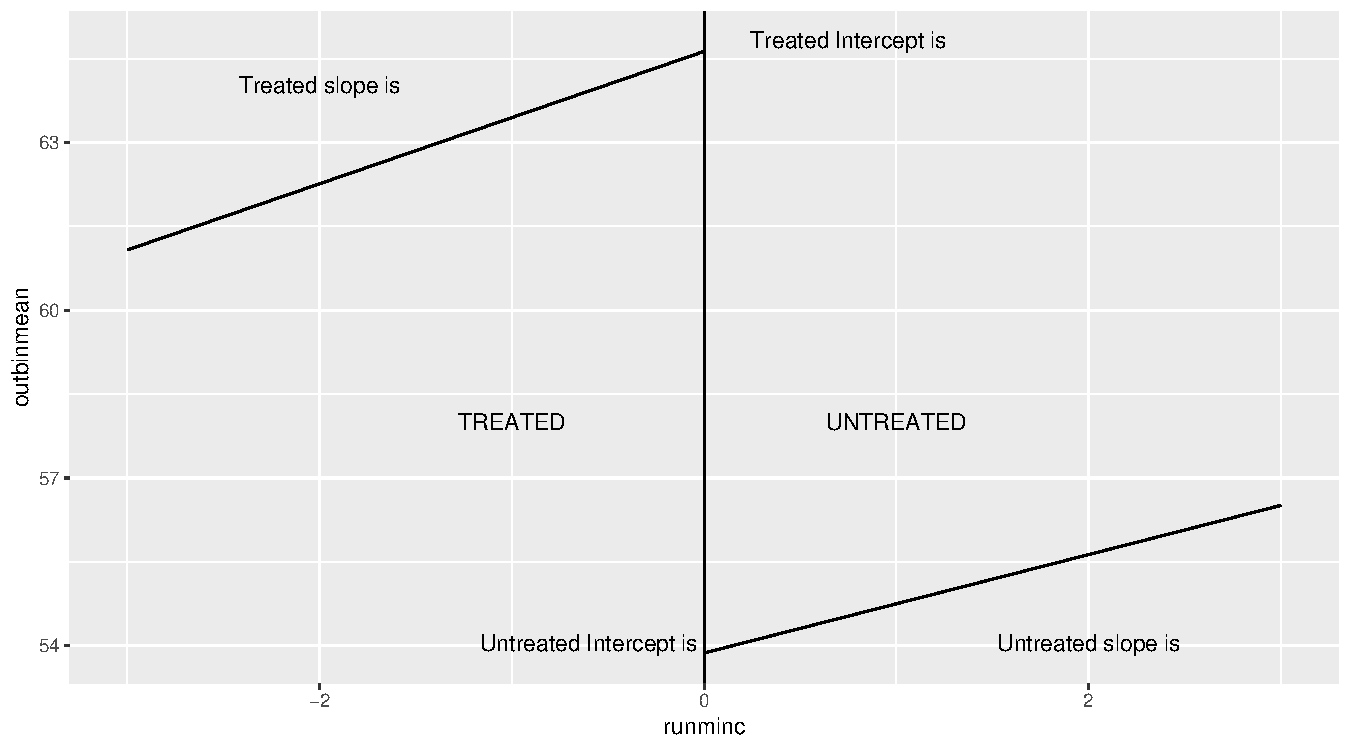
\includegraphics{Slides9_RD_files/figure-beamer/stylea-1.pdf}
\end{frame}

\begin{frame}[fragile]{RD Estimation: Sharp}
\protect\hypertarget{rd-estimation-sharp-3}{}
It is helpful to see how the coefficients estimated above translate to
the RD graph.

\tiny

\begin{Shaded}
\begin{Highlighting}[]
\NormalTok{sharp\_mean}\SpecialCharTok{$}\NormalTok{runminc}\OtherTok{\textless{}{-}}\NormalTok{sharp\_mean}\SpecialCharTok{$}\NormalTok{bins}\DecValTok{{-}75}

\NormalTok{plot6shp}\OtherTok{\textless{}{-}}\FunctionTok{ggplot}\NormalTok{(sharp\_mean, }\FunctionTok{aes}\NormalTok{(}\AttributeTok{x=}\NormalTok{runminc, }\AttributeTok{y=}\NormalTok{outbinmean))}\SpecialCharTok{+} 
         \FunctionTok{geom\_point}\NormalTok{()}\SpecialCharTok{+}
         \FunctionTok{geom\_vline}\NormalTok{(}\AttributeTok{xintercept =} \DecValTok{0}\NormalTok{)}\SpecialCharTok{+}
         \FunctionTok{geom\_segment}\NormalTok{(}\FunctionTok{aes}\NormalTok{(}\AttributeTok{x =} \DecValTok{0}\NormalTok{, }\AttributeTok{xend =} \DecValTok{3}\NormalTok{, }
                          \AttributeTok{y =}\NormalTok{ shpestim}\SpecialCharTok{$}\NormalTok{coefficients[}\DecValTok{1}\NormalTok{],}
                          \AttributeTok{yend =}\NormalTok{ shpestim}\SpecialCharTok{$}\NormalTok{coefficients[}\DecValTok{1}\NormalTok{]}
                                 \SpecialCharTok{+}\DecValTok{3}\SpecialCharTok{*}\NormalTok{shpestim}\SpecialCharTok{$}\NormalTok{coefficients[}\DecValTok{3}\NormalTok{]))}\SpecialCharTok{+}
         \FunctionTok{geom\_segment}\NormalTok{(}\FunctionTok{aes}\NormalTok{(}\AttributeTok{x =} \SpecialCharTok{{-}}\DecValTok{3}\NormalTok{, }\AttributeTok{xend =} \DecValTok{0}\NormalTok{,}
                          \AttributeTok{y =}\NormalTok{ shpestim}\SpecialCharTok{$}\NormalTok{coefficients[}\DecValTok{1}\NormalTok{]}
                              \SpecialCharTok{+}\NormalTok{ shpestim}\SpecialCharTok{$}\NormalTok{coefficients[}\DecValTok{2}\NormalTok{]}
                              \SpecialCharTok{+}\NormalTok{(}\SpecialCharTok{{-}}\DecValTok{3}\SpecialCharTok{*}\NormalTok{( shpestim}\SpecialCharTok{$}\NormalTok{coefficients[}\DecValTok{3}\NormalTok{]}\SpecialCharTok{+}\NormalTok{ shpestim}\SpecialCharTok{$}\NormalTok{coefficients[}\DecValTok{4}\NormalTok{])), }
                          \AttributeTok{yend =}\NormalTok{ shpestim}\SpecialCharTok{$}\NormalTok{coefficients[}\DecValTok{1}\NormalTok{]}
                              \SpecialCharTok{+}\NormalTok{ shpestim}\SpecialCharTok{$}\NormalTok{coefficients[}\DecValTok{2}\NormalTok{]))}\SpecialCharTok{+}
          \CommentTok{\#adding some labeling for course notes:}
          \FunctionTok{annotate}\NormalTok{(}\StringTok{"text"}\NormalTok{, }\AttributeTok{x =} \FloatTok{0.75}\NormalTok{, }\AttributeTok{y =} \FloatTok{64.8}\NormalTok{,}
                   \AttributeTok{label =} \StringTok{"Intercept\textasciitilde{}is\textasciitilde{}alpha\textasciitilde{}+\textasciitilde{}tau"}\NormalTok{ ,}\AttributeTok{parse =} \ConstantTok{TRUE}\NormalTok{)}\SpecialCharTok{+}
          \FunctionTok{annotate}\NormalTok{(}\StringTok{"text"}\NormalTok{, }\AttributeTok{x =} \SpecialCharTok{{-}}\FloatTok{0.6}\NormalTok{, }\AttributeTok{y =} \DecValTok{54}\NormalTok{, }
                   \AttributeTok{label =} \StringTok{"Intercept\textasciitilde{}is\textasciitilde{}alpha"}\NormalTok{ ,}\AttributeTok{parse =} \ConstantTok{TRUE}\NormalTok{)}\SpecialCharTok{+}
          \FunctionTok{annotate}\NormalTok{(}\StringTok{"text"}\NormalTok{, }\AttributeTok{x =} \SpecialCharTok{{-}}\DecValTok{2}\NormalTok{, }\AttributeTok{y =} \DecValTok{64}\NormalTok{,}
                   \AttributeTok{label =} \StringTok{"Slope\textasciitilde{}is\textasciitilde{}beta\textasciitilde{}+\textasciitilde{}gamma"}\NormalTok{ ,}\AttributeTok{parse =} \ConstantTok{TRUE}\NormalTok{)}\SpecialCharTok{+}
          \FunctionTok{annotate}\NormalTok{(}\StringTok{"text"}\NormalTok{, }\AttributeTok{x =} \DecValTok{2}\NormalTok{, }\AttributeTok{y =} \DecValTok{54}\NormalTok{, }
                   \AttributeTok{label =} \StringTok{"Slope\textasciitilde{}is\textasciitilde{}beta"}\NormalTok{ ,}\AttributeTok{parse =} \ConstantTok{TRUE}\NormalTok{)}\SpecialCharTok{+}
          \FunctionTok{annotate}\NormalTok{(}\StringTok{"text"}\NormalTok{, }\AttributeTok{x =} \SpecialCharTok{{-}}\DecValTok{1}\NormalTok{, }\AttributeTok{y =} \DecValTok{58}\NormalTok{, }
                   \AttributeTok{label =} \StringTok{"TREATED"}\NormalTok{ ,}\AttributeTok{parse =} \ConstantTok{TRUE}\NormalTok{)}\SpecialCharTok{+}
          \FunctionTok{annotate}\NormalTok{(}\StringTok{"text"}\NormalTok{, }\AttributeTok{x =} \DecValTok{1}\NormalTok{, }\AttributeTok{y =} \DecValTok{58}\NormalTok{, }
                   \AttributeTok{label =} \StringTok{"UNTREATED"}\NormalTok{ ,}\AttributeTok{parse =} \ConstantTok{TRUE}\NormalTok{) }
\end{Highlighting}
\end{Shaded}
\end{frame}

\begin{frame}[fragile]{RD Estimation: Sharp}
\protect\hypertarget{rd-estimation-sharp-4}{}
\[
Y_i=\alpha+\tau D_i+\beta(R_i-c)+\gamma (R_i-c)*D_i+u_i \text{ for }  c-h\leq R_i< c+h. 
\]

\tiny

\begin{Shaded}
\begin{Highlighting}[]
\NormalTok{plot6shp}
\end{Highlighting}
\end{Shaded}

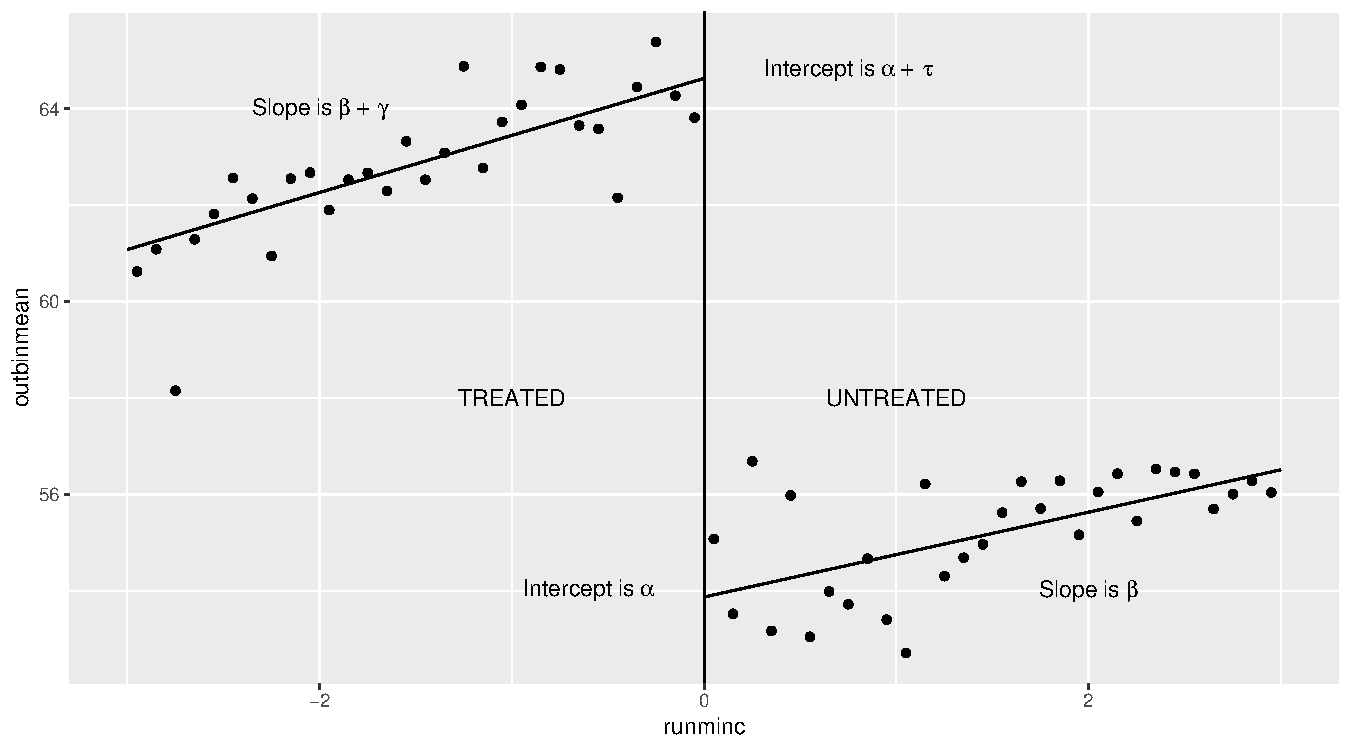
\includegraphics{Slides9_RD_files/figure-beamer/shp7b-1.pdf}
\end{frame}

\hypertarget{fuzzy-rd}{%
\section{Fuzzy RD}\label{fuzzy-rd}}

\begin{frame}{Fuzzy RD Set Up}
\protect\hypertarget{fuzzy-rd-set-up}{}
Potentially more common than the sharp RD set ups.

\(D_i\) is no longer a deterministic function of \(R_i\).

The probability of treatment changes by some nonzero amount as the
running variable crosses the threshold \(c\).

The change in probability is less than 100 percentage points.

\[
0<\lim\limits_{r\rightarrow c}P(D_i=1|R_i=r)-\lim\limits_{r\leftarrow c}P(D_i=1|R_i=r)<1
\]
\end{frame}

\begin{frame}{Fuzzy RD Set Up}
\protect\hypertarget{fuzzy-rd-set-up-1}{}
There are now two causal effects to be estimated:

\begin{itemize}
\item
  the effect of crossing the threshold on the probability of treatment
  (which is 1 in the sharp RD)
\item
  the effect of crossing the threshold on the outcome.
\end{itemize}

Formally, the fuzzy RD estimator is

\[
\tau_{FRD}=\frac{\lim\limits_{r\rightarrow c} E[Y_i|R_i=r]-\lim\limits_{r\leftarrow c}E[Y_i|R_i=r]}{\lim\limits_{r\rightarrow c} E[D_i|R_i=r]-\lim\limits_{r\leftarrow c}E[D_i|R_i=r]}.
\]

\textbf{What should this remind you of?}
\end{frame}

\begin{frame}{Fuzzy RD IV}
\protect\hypertarget{fuzzy-rd-iv}{}
RD analog of an IV estimator:

\begin{itemize}
\item
  the instrument is an indicator for whether \(R_i\) lies directly
  above(below) \(c\).
\item
  similar to how the IV estimator allowed us to recover the LATE
  estimate in an RCT.
\end{itemize}

-you (randomly) fall above (below) c which changes the probability of
treatment. We leverage this change in probability as an instrument to
estimate the effect of treatment on the outcome.
\end{frame}

\begin{frame}{Fuzzy RD IV}
\protect\hypertarget{fuzzy-rd-iv-1}{}
In a fuzzy RD:

\begin{itemize}
\item
  the ITT group (say who have \(R_i\leq c\) for example)
\item
  the control group (\(R_i>c\)).
\end{itemize}

Because we are in fuzzy land:

\begin{itemize}
\item
  being in the ITT group does not necessarily mean you get treated
  (there are never takers)
\item
  some in the control get treated (always takers).
\item
  but there is a group of observations, the compliers, whose treatment
  status changes if they go from control to ITT (ie if they were moved
  across the threshold).
\end{itemize}
\end{frame}

\begin{frame}{Fuzzy RD IV}
\protect\hypertarget{fuzzy-rd-iv-2}{}
If I just compare the outcomes of those that are above and below the
threshold
(\(\lim\limits_{r\rightarrow c} E[Y_i|R_i=r]-\lim\limits_{r\leftarrow c}E[Y_i|R_i=r]\))
the effect is ``diluted''. \textbf{Why?}
\end{frame}

\begin{frame}{Fuzzy RD IV}
\protect\hypertarget{fuzzy-rd-iv-3}{}
If I just compare the outcomes of those that are above and below the
threshold
(\(\lim\limits_{r\rightarrow c} E[Y_i|R_i=r]-\lim\limits_{r\leftarrow c}E[Y_i|R_i=r]\))
the effect is ``diluted''. \textbf{Why?}

\begin{itemize}
\tightlist
\item
  for many observations, crossing the threshold has no effect (since
  they are always or never takers).
\end{itemize}
\end{frame}

\begin{frame}{Fuzzy RD IV}
\protect\hypertarget{fuzzy-rd-iv-4}{}
To get the LATE, scale treatment estimates by the change in probability
of being treated
(\(\lim\limits_{r\rightarrow c} E[D_i|R_i=r]-\lim\limits_{r\leftarrow c}E[D_i|R_i=r]\)).

\(\Rightarrow\) the fuzzy RD design measures the average treatment
effect for RD compliers at the threshold (the LATE), \[
\tau_{FRD}=E[Y_i(1)-Y_i(0)|\text{unit }i\text{ is a complier and } R_i=c]. 
\]
\end{frame}

\begin{frame}{Fuzzy RD Simulation:}
\protect\hypertarget{fuzzy-rd-simulation}{}
You are the superintendent of a large school district.

Last year you \textbf{strongly encouraged} students to participate in
small reading groups if their 3rd grade reading score fell below 75
points.

Your data includes the 3rd and 4th grade reading scores for all 5000
students in your school district.

\textbf{How did these reading groups affected student performance on
their 4th grade reading tests?}
\end{frame}

\begin{frame}[fragile]{Fuzzy RD Simulation:}
\protect\hypertarget{fuzzy-rd-simulation-1}{}
\tiny

\begin{Shaded}
\begin{Highlighting}[]
\FunctionTok{set.seed}\NormalTok{(}\DecValTok{2000}\NormalTok{)}

\NormalTok{fuzzy}\OtherTok{\textless{}{-}}\FunctionTok{rnorm}\NormalTok{(}\DecValTok{5000}\NormalTok{, }\AttributeTok{mean=}\DecValTok{80}\NormalTok{, }\AttributeTok{sd=}\DecValTok{5}\NormalTok{)}
\NormalTok{fuzzy}\OtherTok{\textless{}{-}}\FunctionTok{as.data.frame}\NormalTok{(fuzzy)}

\FunctionTok{names}\NormalTok{(fuzzy)}\OtherTok{\textless{}{-}}\FunctionTok{c}\NormalTok{(}\StringTok{"read3"}\NormalTok{)}
\NormalTok{fuzzy}\SpecialCharTok{$}\NormalTok{error}\OtherTok{\textless{}{-}}\FunctionTok{rnorm}\NormalTok{(}\DecValTok{5000}\NormalTok{, }\AttributeTok{mean=}\DecValTok{0}\NormalTok{, }\AttributeTok{sd=}\DecValTok{5}\NormalTok{)}
\NormalTok{fuzzy}\SpecialCharTok{$}\NormalTok{pe3}\OtherTok{\textless{}{-}}\FunctionTok{rnorm}\NormalTok{(}\DecValTok{5000}\NormalTok{, }\AttributeTok{mean=}\DecValTok{90}\NormalTok{, }\AttributeTok{sd=}\DecValTok{4}\NormalTok{)}
\NormalTok{fuzzy}\SpecialCharTok{$}\NormalTok{height}\OtherTok{\textless{}{-}}\FunctionTok{rnorm}\NormalTok{(}\DecValTok{5000}\NormalTok{, }\AttributeTok{mean=}\DecValTok{130}\NormalTok{, }\AttributeTok{sd=}\DecValTok{15}\NormalTok{)}



\NormalTok{fuzzy}\SpecialCharTok{$}\NormalTok{lowprob}\OtherTok{\textless{}{-}}\FunctionTok{rbinom}\NormalTok{(}\DecValTok{5000}\NormalTok{,}\DecValTok{1}\NormalTok{,}\FloatTok{0.3}\NormalTok{)}
\NormalTok{fuzzy}\SpecialCharTok{$}\NormalTok{highprob}\OtherTok{\textless{}{-}}\FunctionTok{rbinom}\NormalTok{(}\DecValTok{5000}\NormalTok{,}\DecValTok{1}\NormalTok{,}\FloatTok{0.8}\NormalTok{)}
\NormalTok{fuzzy}\SpecialCharTok{$}\NormalTok{treated}\OtherTok{\textless{}{-}}\ConstantTok{NA}
\NormalTok{fuzzy}\SpecialCharTok{$}\NormalTok{treated[fuzzy}\SpecialCharTok{$}\NormalTok{read3}\SpecialCharTok{\textgreater{}}\DecValTok{75}\NormalTok{]}\OtherTok{\textless{}{-}}\NormalTok{fuzzy}\SpecialCharTok{$}\NormalTok{lowprob[fuzzy}\SpecialCharTok{$}\NormalTok{read3}\SpecialCharTok{\textgreater{}}\DecValTok{75}\NormalTok{]}
\NormalTok{fuzzy}\SpecialCharTok{$}\NormalTok{treated[fuzzy}\SpecialCharTok{$}\NormalTok{read3}\SpecialCharTok{\textless{}=}\DecValTok{75}\NormalTok{]}\OtherTok{\textless{}{-}}\NormalTok{fuzzy}\SpecialCharTok{$}\NormalTok{highprob[fuzzy}\SpecialCharTok{$}\NormalTok{read3}\SpecialCharTok{\textless{}=}\DecValTok{75}\NormalTok{]}

\NormalTok{tau}\OtherTok{=}\DecValTok{10}

\CommentTok{\#the DGP}
\NormalTok{fuzzy}\SpecialCharTok{$}\NormalTok{read4}\OtherTok{\textless{}{-}}\NormalTok{(}\SpecialCharTok{{-}}\DecValTok{6}\NormalTok{)}\SpecialCharTok{+}\FloatTok{0.8}\SpecialCharTok{*}\NormalTok{fuzzy}\SpecialCharTok{$}\NormalTok{read3}\SpecialCharTok{+}\NormalTok{tau}\SpecialCharTok{*}\NormalTok{fuzzy}\SpecialCharTok{$}\NormalTok{treated}\SpecialCharTok{+}\NormalTok{fuzzy}\SpecialCharTok{$}\NormalTok{error}

\NormalTok{fuzzy}\OtherTok{\textless{}{-}}\NormalTok{fuzzy[fuzzy}\SpecialCharTok{$}\NormalTok{read3}\SpecialCharTok{\textless{}}\DecValTok{78} \SpecialCharTok{\&}\NormalTok{ fuzzy}\SpecialCharTok{$}\NormalTok{read3}\SpecialCharTok{\textgreater{}}\DecValTok{72}\NormalTok{,]}
\end{Highlighting}
\end{Shaded}
\end{frame}

\begin{frame}{Fuzzy RD: Treatment status graph}
\protect\hypertarget{fuzzy-rd-treatment-status-graph}{}
We calculate \(\bar{D}_k\), the average treatment level in the bin

\[
\bar{D}_k=\frac{1}{N_k}\sum_{i=1}^ND_i*\mathbf{1}(b_k<R_i\leq b_{k+1}).
\]

In a fuzzy RD, \(\bar{D}_k\) can take on many possible values.

This plot should show that there is a visual discontinuity in the
probability of getting treated at the threshold \(c\).

This graph is equivalent to the first stage in an IV analysis: It shows
that we have found a tool that generates some random variation we can
leverage to estimate unbiased treatment effects.
\end{frame}

\begin{frame}[fragile]{Fuzzy RD: Treatment status graph Simulation}
\protect\hypertarget{fuzzy-rd-treatment-status-graph-simulation}{}
\tiny

\begin{Shaded}
\begin{Highlighting}[]
\CommentTok{\#I will break up the data into 60 bins (30 above and 30 below the threshold)}

\NormalTok{cuts}\OtherTok{\textless{}{-}}\FunctionTok{c}\NormalTok{(}\DecValTok{72}\NormalTok{,}\FloatTok{72.1}\NormalTok{,}\FloatTok{72.2}\NormalTok{,}\FloatTok{72.3}\NormalTok{,}\FloatTok{72.4}\NormalTok{,}\FloatTok{72.5}\NormalTok{,}\FloatTok{72.6}\NormalTok{,}\FloatTok{72.7}\NormalTok{,}\FloatTok{72.8}\NormalTok{,}\FloatTok{72.9}\NormalTok{,}\DecValTok{73}\NormalTok{,}
        \FloatTok{73.1}\NormalTok{,}\FloatTok{73.2}\NormalTok{,}\FloatTok{73.3}\NormalTok{,}\FloatTok{73.4}\NormalTok{,}\FloatTok{73.5}\NormalTok{,}\FloatTok{73.6}\NormalTok{,}\FloatTok{73.7}\NormalTok{,}\FloatTok{73.8}\NormalTok{,}\FloatTok{73.9}\NormalTok{,}\DecValTok{74}\NormalTok{,}
        \FloatTok{74.1}\NormalTok{,}\FloatTok{74.2}\NormalTok{,}\FloatTok{74.3}\NormalTok{,}\FloatTok{74.4}\NormalTok{,}\FloatTok{74.5}\NormalTok{,}\FloatTok{74.6}\NormalTok{,}\FloatTok{74.7}\NormalTok{,}\FloatTok{74.8}\NormalTok{,}\FloatTok{74.9}\NormalTok{,}\DecValTok{75}\NormalTok{,}
        \FloatTok{75.1}\NormalTok{,}\FloatTok{75.2}\NormalTok{,}\FloatTok{75.3}\NormalTok{,}\FloatTok{75.4}\NormalTok{,}\FloatTok{75.5}\NormalTok{,}\FloatTok{75.6}\NormalTok{,}\FloatTok{75.7}\NormalTok{,}\FloatTok{75.8}\NormalTok{,}\FloatTok{75.9}\NormalTok{,}\DecValTok{76}\NormalTok{,}
        \FloatTok{76.1}\NormalTok{,}\FloatTok{76.2}\NormalTok{,}\FloatTok{76.3}\NormalTok{,}\FloatTok{76.4}\NormalTok{,}\FloatTok{76.5}\NormalTok{,}\FloatTok{76.6}\NormalTok{,}\FloatTok{76.7}\NormalTok{,}\FloatTok{76.8}\NormalTok{,}\FloatTok{76.9}\NormalTok{,}\DecValTok{77}\NormalTok{,}
        \FloatTok{77.1}\NormalTok{,}\FloatTok{77.2}\NormalTok{,}\FloatTok{77.3}\NormalTok{,}\FloatTok{77.4}\NormalTok{,}\FloatTok{77.5}\NormalTok{,}\FloatTok{77.6}\NormalTok{,}\FloatTok{77.7}\NormalTok{,}\FloatTok{77.8}\NormalTok{,}\FloatTok{77.9}\NormalTok{,}\DecValTok{78}\NormalTok{)}
\NormalTok{midpoints}\OtherTok{\textless{}{-}}\NormalTok{cuts[}\DecValTok{2}\SpecialCharTok{:}\DecValTok{61}\NormalTok{]}\SpecialCharTok{{-}}\FloatTok{0.05}

\NormalTok{fuzzy}\SpecialCharTok{$}\NormalTok{bins }\OtherTok{\textless{}{-}} \FunctionTok{cut}\NormalTok{(fuzzy}\SpecialCharTok{$}\NormalTok{read3, }
                  \AttributeTok{breaks=}\NormalTok{cuts, }
                  \AttributeTok{include.lowest=}\ConstantTok{TRUE}\NormalTok{, }
                  \AttributeTok{right=}\ConstantTok{FALSE}\NormalTok{, }
                  \AttributeTok{labels=}\NormalTok{midpoints)}
        

\NormalTok{fuzzy\_mean}\OtherTok{\textless{}{-}}\NormalTok{fuzzy }\SpecialCharTok{\%\textgreater{}\%}
    \FunctionTok{group\_by}\NormalTok{(bins) }\SpecialCharTok{\%\textgreater{}\%}
\NormalTok{    dplyr}\SpecialCharTok{::}\FunctionTok{summarize}\NormalTok{(}\AttributeTok{outbinmean =} \FunctionTok{mean}\NormalTok{(read4, }\AttributeTok{na.rm=}\ConstantTok{TRUE}\NormalTok{),}
                     \AttributeTok{treatbinmean=}\FunctionTok{mean}\NormalTok{(treated, }\AttributeTok{na.rm=}\ConstantTok{TRUE}\NormalTok{),}
                     \AttributeTok{pebinmean=}\FunctionTok{mean}\NormalTok{(pe3, }\AttributeTok{na.rm=}\ConstantTok{TRUE}\NormalTok{),}
                     \AttributeTok{heightbinmean=}\FunctionTok{mean}\NormalTok{(height, }\AttributeTok{na.rm=}\ConstantTok{TRUE}\NormalTok{), }\AttributeTok{numb=}\FunctionTok{n}\NormalTok{())}

\NormalTok{fuzzy\_mean}\SpecialCharTok{$}\NormalTok{bins}\OtherTok{\textless{}{-}}\FunctionTok{as.numeric}\NormalTok{(}\FunctionTok{as.character}\NormalTok{(fuzzy\_mean}\SpecialCharTok{$}\NormalTok{bins))}

\NormalTok{plot1fuz}\OtherTok{\textless{}{-}}\FunctionTok{ggplot}\NormalTok{(fuzzy\_mean, }\FunctionTok{aes}\NormalTok{(}\AttributeTok{x=}\NormalTok{bins, }\AttributeTok{y=}\NormalTok{treatbinmean))}\SpecialCharTok{+} 
         \FunctionTok{geom\_point}\NormalTok{()}\SpecialCharTok{+}
         \FunctionTok{geom\_vline}\NormalTok{(}\AttributeTok{xintercept =} \DecValTok{75}\NormalTok{)}
\end{Highlighting}
\end{Shaded}
\end{frame}

\begin{frame}[fragile]{Fuzzy RD: Treatment status graph Simulation}
\protect\hypertarget{fuzzy-rd-treatment-status-graph-simulation-1}{}
\begin{Shaded}
\begin{Highlighting}[]
\NormalTok{plot1fuz}
\end{Highlighting}
\end{Shaded}

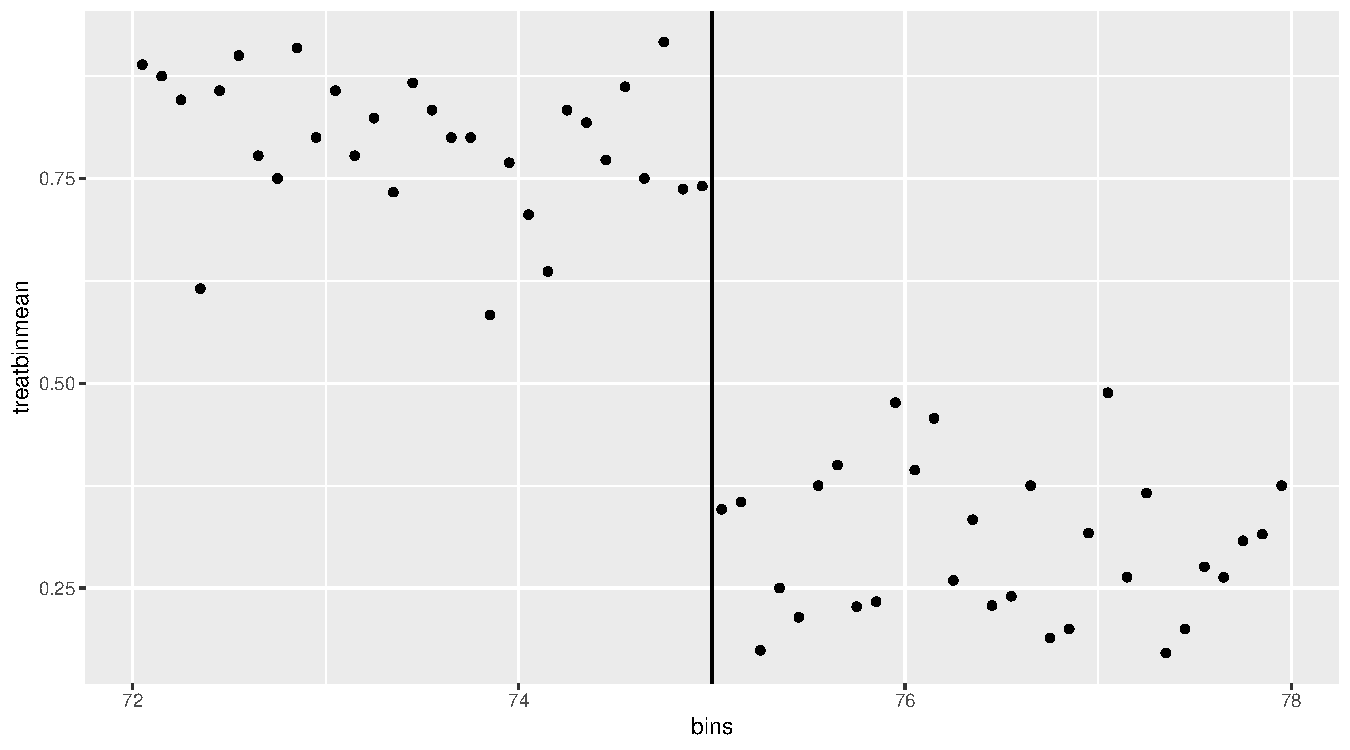
\includegraphics{Slides9_RD_files/figure-beamer/fuzzy2a-1.pdf}
\end{frame}

\begin{frame}[fragile]{Outcome Graphs: Fuzzy}
\protect\hypertarget{outcome-graphs-fuzzy}{}
In the earlier chunk, we calculated, \(\bar{Y}_k\), the average outcome
in each bin

\[
\bar{Y}_k=\frac{1}{N_k}\sum_{i=1}^NY_i*\mathbf{1}(b_k<R_i\leq b_{k+1})
\]

\begin{Shaded}
\begin{Highlighting}[]
\NormalTok{plot2fuz}\OtherTok{\textless{}{-}}\FunctionTok{ggplot}\NormalTok{(fuzzy\_mean, }\FunctionTok{aes}\NormalTok{(}\AttributeTok{x=}\NormalTok{bins, }\AttributeTok{y=}\NormalTok{outbinmean))}\SpecialCharTok{+} 
         \FunctionTok{geom\_point}\NormalTok{()}\SpecialCharTok{+}
         \FunctionTok{geom\_vline}\NormalTok{(}\AttributeTok{xintercept =} \DecValTok{75}\NormalTok{)}
\end{Highlighting}
\end{Shaded}
\end{frame}

\begin{frame}{Outcome Graphs: Fuzzy}
\protect\hypertarget{outcome-graphs-fuzzy-1}{}
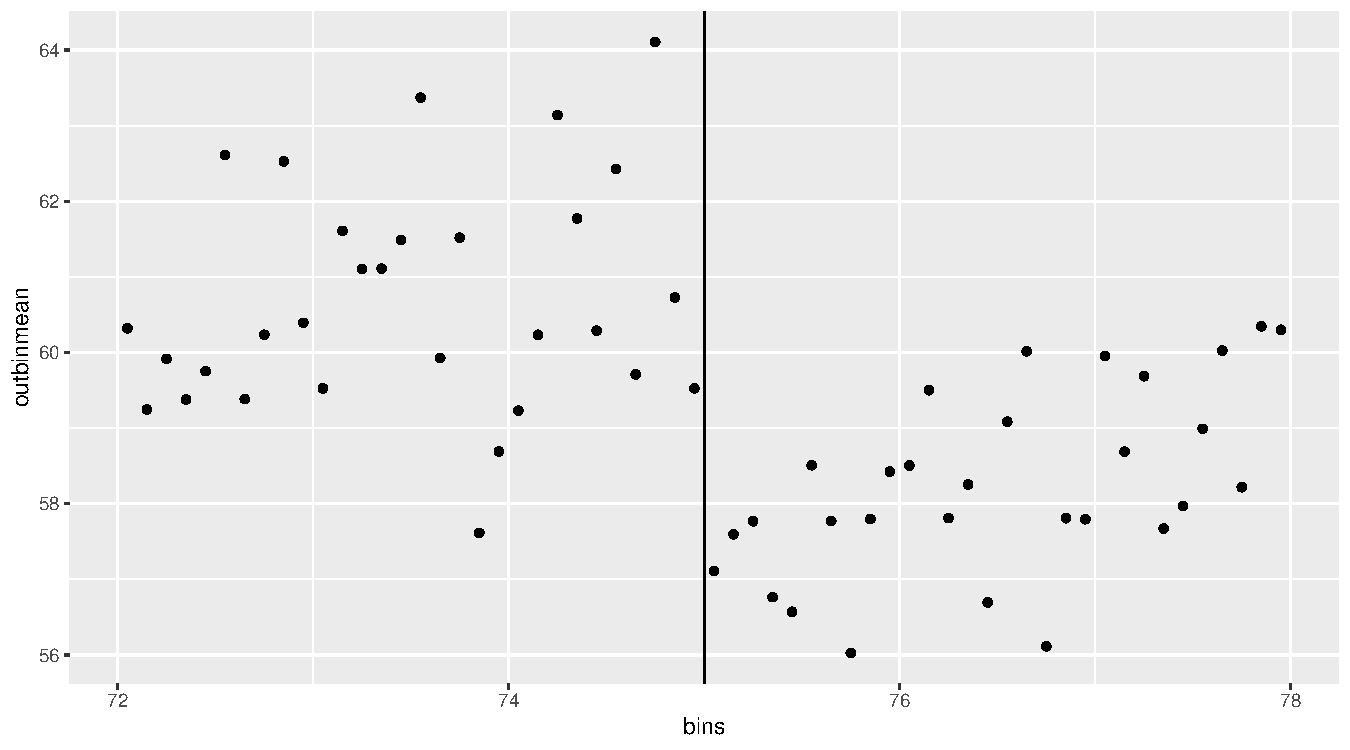
\includegraphics{Slides9_RD_files/figure-beamer/fuz3b-1.pdf}
\end{frame}

\begin{frame}[fragile]{Robustness Graphs: Covariates fuzzy}
\protect\hypertarget{robustness-graphs-covariates-fuzzy}{}
In the earlier chunk, we calculated \(\bar{X}_k\) where \[
\bar{X}_k=\frac{1}{N_k}\sum_{i=1}^NX_i*\mathbf{1}(b_k<R_i\leq b_{k+1})
\]

\tiny

\begin{Shaded}
\begin{Highlighting}[]
\NormalTok{plot3fuz}\OtherTok{\textless{}{-}}\FunctionTok{ggplot}\NormalTok{(fuzzy\_mean, }\FunctionTok{aes}\NormalTok{(}\AttributeTok{x=}\NormalTok{bins, }\AttributeTok{y=}\NormalTok{pebinmean))}\SpecialCharTok{+} 
         \FunctionTok{geom\_point}\NormalTok{()}\SpecialCharTok{+}
         \FunctionTok{geom\_vline}\NormalTok{(}\AttributeTok{xintercept =} \DecValTok{75}\NormalTok{)}
\end{Highlighting}
\end{Shaded}
\end{frame}

\begin{frame}{Robustness Graphs: Covariates fuzzy}
\protect\hypertarget{robustness-graphs-covariates-fuzzy-1}{}
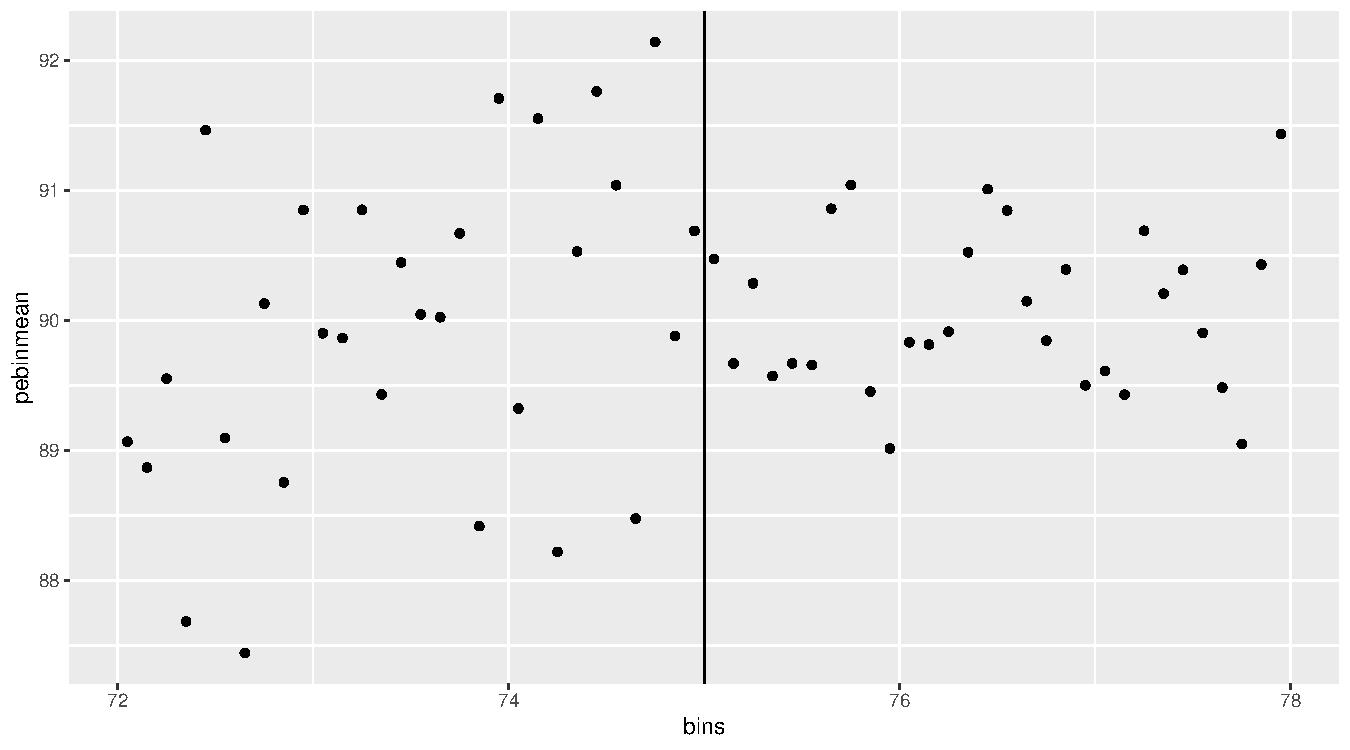
\includegraphics{Slides9_RD_files/figure-beamer/fuz4aa-1.pdf}
\end{frame}

\begin{frame}{Robustness Graphs: Covariates fuzzy}
\protect\hypertarget{robustness-graphs-covariates-fuzzy-2}{}
\tiny

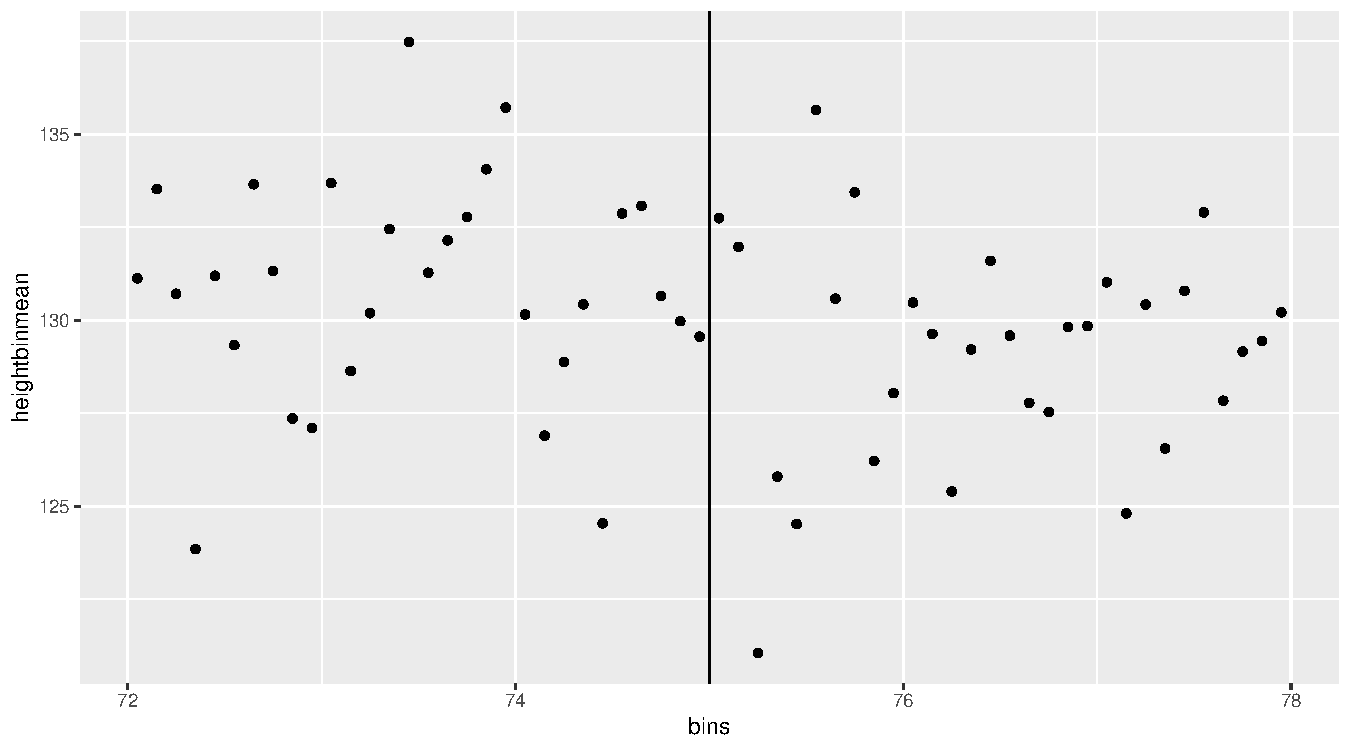
\includegraphics{Slides9_RD_files/figure-beamer/fuz4b-1.pdf}
\end{frame}

\begin{frame}[fragile]{Robustness Graphs: Density of the Running
Variable (Fuzzy)}
\protect\hypertarget{robustness-graphs-density-of-the-running-variable-fuzzy}{}
In an earlier chunk we calculated \[
N_k=\sum_{i=1}^N\mathbf{1}(b_k<R_i\leq b_{k+1})
\]

\tiny

\begin{Shaded}
\begin{Highlighting}[]
\NormalTok{plot5fuz}\OtherTok{\textless{}{-}}\FunctionTok{ggplot}\NormalTok{(fuzzy\_mean, }\FunctionTok{aes}\NormalTok{(}\AttributeTok{x=}\NormalTok{bins, }\AttributeTok{y=}\NormalTok{numb))}\SpecialCharTok{+} 
         \FunctionTok{geom\_point}\NormalTok{()}\SpecialCharTok{+}
         \FunctionTok{geom\_vline}\NormalTok{(}\AttributeTok{xintercept =} \DecValTok{75}\NormalTok{)}
\end{Highlighting}
\end{Shaded}
\end{frame}

\begin{frame}[fragile]{Robustness Graphs: Density of the Running
Variable (Fuzzy)}
\protect\hypertarget{robustness-graphs-density-of-the-running-variable-fuzzy-1}{}
\begin{Shaded}
\begin{Highlighting}[]
\NormalTok{plot5fuz}
\end{Highlighting}
\end{Shaded}

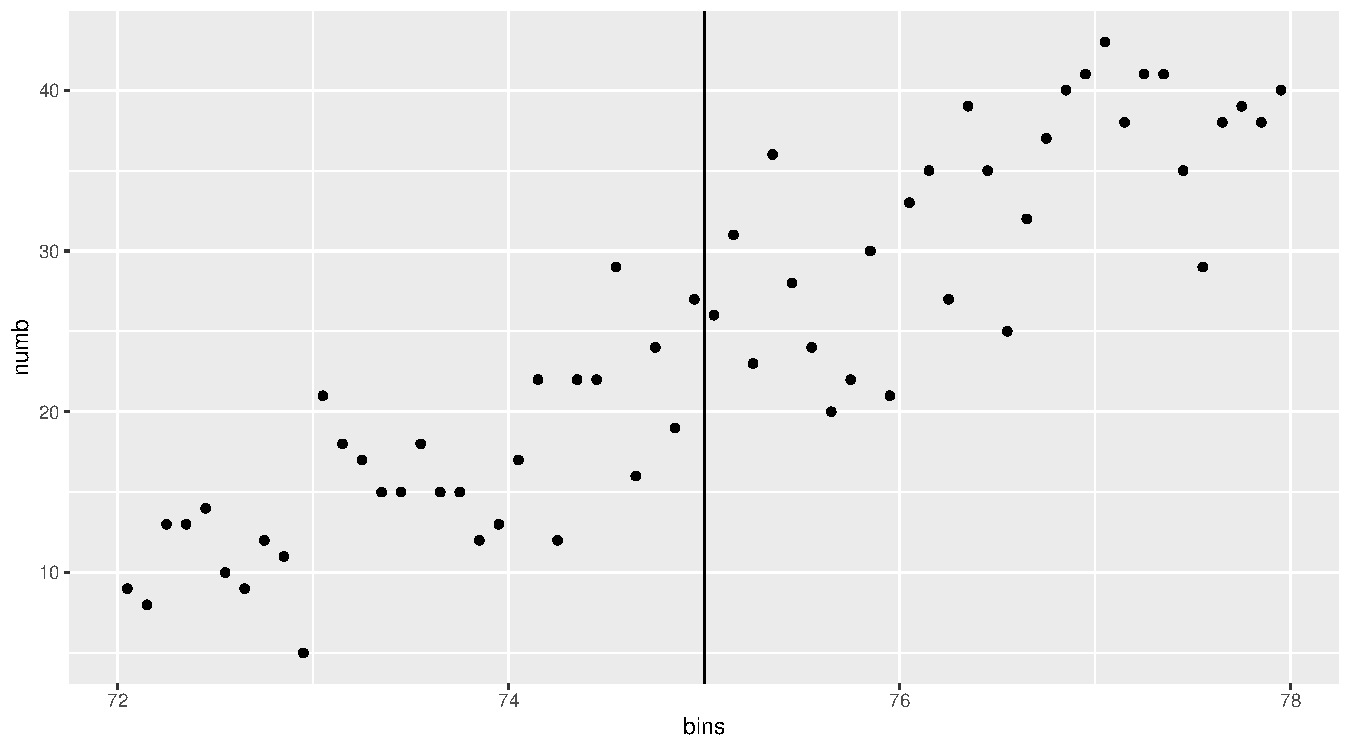
\includegraphics{Slides9_RD_files/figure-beamer/fuz5a-1.pdf}
\end{frame}

\begin{frame}{RD Estimation: Fuzzy}
\protect\hypertarget{rd-estimation-fuzzy}{}
In the fuzzy RD design, we have two effects to estimate:

\begin{itemize}
\item
  the effect of crossing the threshold on the treatment (the ``first
  stage'')
\item
  the effect of crossing the threshold on the outcome (the ``reduced
  form'').
\end{itemize}

We apply the same methodology as in earlier IV's to estimate the effect
of crossing the threshold on \(Y_i\) and the effect of crossing the
threshold on \(D_i\).
\end{frame}

\begin{frame}{RD Estimation: Fuzzy}
\protect\hypertarget{rd-estimation-fuzzy-1}{}
For the sample with \(c-h \leq R_i< c+h\) we run some version (you can
include covariates) of the following ``reduced form'' IV regression \[
Y_i=\pi_0+\pi_1Z_i+\pi_2(R_i-c)+\pi_3(R_i-c)*Z_i+u_i 
\] where the first stage is given by \[
D_i=\gamma_0+\gamma_1Z_i+\gamma_2(R_i-c)+\gamma_3(R_i-c)*Z_i+v_i
\] where \(Z_i=1(R_i> c)\).
\end{frame}

\begin{frame}{RD Estimation: Fuzzy}
\protect\hypertarget{rd-estimation-fuzzy-2}{}
The fuzzy RD estimator is then

\[
\hat{\tau}_{FRD}=\frac{\hat{\pi}_1}{\hat{\gamma}_1}.
\] The FRD estimator is the ratio of the reduced form and the first
stage estimates (aka the IV estimator).

i.e.~the effect of crossing the discontinuity threshold on the outcome,
scaled by the effect of crossing the discontinuity threshold on the
probability of treatment.
\end{frame}

\begin{frame}[fragile]{RD Estimation: Fuzzy}
\protect\hypertarget{rd-estimation-fuzzy-3}{}
\tiny

\begin{Shaded}
\begin{Highlighting}[]
\NormalTok{fuzzy}\SpecialCharTok{$}\NormalTok{runminc}\OtherTok{\textless{}{-}}\NormalTok{fuzzy}\SpecialCharTok{$}\NormalTok{read3}\DecValTok{{-}75}

\CommentTok{\#first stage}
\NormalTok{fuzzy}\SpecialCharTok{$}\NormalTok{ittgroup}\OtherTok{\textless{}{-}}\DecValTok{0}
\NormalTok{fuzzy}\SpecialCharTok{$}\NormalTok{ittgroup[fuzzy}\SpecialCharTok{$}\NormalTok{read3}\SpecialCharTok{\textless{}=}\DecValTok{75}\NormalTok{]}\OtherTok{\textless{}{-}}\DecValTok{1}

\NormalTok{fuzfs}\OtherTok{\textless{}{-}}\FunctionTok{felm}\NormalTok{(treated}\SpecialCharTok{\textasciitilde{}}\NormalTok{ittgroup}\SpecialCharTok{+}\NormalTok{runminc}\SpecialCharTok{+}\NormalTok{ittgroup}\SpecialCharTok{*}\NormalTok{runminc,fuzzy)}

\CommentTok{\#reduced form}
\NormalTok{fuzrf}\OtherTok{\textless{}{-}}\FunctionTok{felm}\NormalTok{(read4}\SpecialCharTok{\textasciitilde{}}\NormalTok{ittgroup}\SpecialCharTok{+}\NormalTok{runminc}\SpecialCharTok{+}\NormalTok{ittgroup}\SpecialCharTok{*}\NormalTok{runminc,fuzzy)}


\NormalTok{fuzzy}\SpecialCharTok{$}\NormalTok{interedog}\OtherTok{\textless{}{-}}\NormalTok{fuzzy}\SpecialCharTok{$}\NormalTok{treated}\SpecialCharTok{*}\NormalTok{fuzzy}\SpecialCharTok{$}\NormalTok{runminc}
\NormalTok{fuzzy}\SpecialCharTok{$}\NormalTok{interinst}\OtherTok{\textless{}{-}}\NormalTok{fuzzy}\SpecialCharTok{$}\NormalTok{ittgroup}\SpecialCharTok{*}\NormalTok{fuzzy}\SpecialCharTok{$}\NormalTok{runminc}
\CommentTok{\#IV}
\NormalTok{fuziv}\OtherTok{\textless{}{-}}\FunctionTok{felm}\NormalTok{(read4}\SpecialCharTok{\textasciitilde{}}\NormalTok{runminc}\SpecialCharTok{|}\DecValTok{0}\SpecialCharTok{|}\NormalTok{(treated}\SpecialCharTok{|}\NormalTok{interedog}\SpecialCharTok{\textasciitilde{}}\NormalTok{ittgroup}\SpecialCharTok{+}\NormalTok{runminc}\SpecialCharTok{+}\NormalTok{interinst),fuzzy)}
\end{Highlighting}
\end{Shaded}

\begin{verbatim}
## Warning in chol.default(mat, pivot = TRUE, tol = tol): the matrix is either
## rank-deficient or indefinite
\end{verbatim}
\end{frame}

\begin{frame}[fragile]{RD Estimation: Fuzzy}
\protect\hypertarget{rd-estimation-fuzzy-4}{}
\tiny

\begin{Shaded}
\begin{Highlighting}[]
\FunctionTok{stargazer}\NormalTok{(fuzfs, fuzrf, fuziv, }\AttributeTok{type=}\StringTok{"latex"}\NormalTok{, }\AttributeTok{header=}\ConstantTok{FALSE}\NormalTok{)}
\end{Highlighting}
\end{Shaded}

\begin{table}[!htbp] \centering 
  \caption{} 
  \label{} 
\begin{tabular}{@{\extracolsep{5pt}}lccc} 
\\[-1.8ex]\hline 
\hline \\[-1.8ex] 
 & \multicolumn{3}{c}{\textit{Dependent variable:}} \\ 
\cline{2-4} 
\\[-1.8ex] & treated & \multicolumn{2}{c}{read4} \\ 
\\[-1.8ex] & (1) & (2) & (3)\\ 
\hline \\[-1.8ex] 
 ittgroup & 0.464$^{***}$ & 4.253$^{***}$ &  \\ 
  & (0.048) & (0.722) &  \\ 
  & & & \\ 
 runminc & $-$0.004 & 0.821$^{***}$ & 1.057$^{***}$ \\ 
  & (0.017) & (0.251) & (0.332) \\ 
  & & & \\ 
 ittgroup:runminc & $-$0.013 & $-$0.479 &  \\ 
  & (0.029) & (0.441) &  \\ 
  & & & \\ 
 `treated(fit)` &  &  & 9.201$^{***}$ \\ 
  &  &  & (1.162) \\ 
  & & & \\ 
 `interedog(fit)` &  &  & $-$0.685 \\ 
  &  &  & (0.631) \\ 
  & & & \\ 
 Constant & 0.308$^{***}$ & 57.010$^{***}$ & 54.182$^{***}$ \\ 
  & (0.030) & (0.460) & (0.640) \\ 
  & & & \\ 
\hline \\[-1.8ex] 
Observations & 1,460 & 1,460 & 1,460 \\ 
R$^{2}$ & 0.213 & 0.037 & 0.454 \\ 
Adjusted R$^{2}$ & 0.211 & 0.035 & 0.453 \\ 
Residual Std. Error (df = 1456) & 0.443 & 6.728 & 5.065 \\ 
\hline 
\hline \\[-1.8ex] 
\textit{Note:}  & \multicolumn{3}{r}{$^{*}$p$<$0.1; $^{**}$p$<$0.05; $^{***}$p$<$0.01} \\ 
\end{tabular} 
\end{table}
\end{frame}

\begin{frame}{RD Estimation: Fuzzy}
\protect\hypertarget{rd-estimation-fuzzy-5}{}
Note: you will not be able to plot the ``scaled'' treatment effect as
the graphs are limited to the graphical equivalent of the first stage
and the reduced form estimates.
\end{frame}

\begin{frame}{RD and External Validity}
\protect\hypertarget{rd-and-external-validity}{}
Notice the conditioning statements in our treatment estimators.

\[
\tau_{SRD}=E[Y_i(1)-Y_i(0)|R_i=c]
\]

\[
\tau_{FRD}=E[Y_i(1)-Y_i(0)|\text{unit }i\text{ is a complier and } R_i=c]. 
\]
\end{frame}

\begin{frame}{RD and External Validity}
\protect\hypertarget{rd-and-external-validity-1}{}
\begin{itemize}
\tightlist
\item
  We focus on observations that are in the neighborhood of the
  threshold. \textbf{Why?}
\end{itemize}
\end{frame}

\begin{frame}{RD and External Validity}
\protect\hypertarget{rd-and-external-validity-2}{}
\begin{itemize}
\tightlist
\item
  We focus on observations that are in the neighborhood of the
  threshold. \textbf{Why?}

  \begin{itemize}
  \tightlist
  \item
    implicitly we are assuming that an observation falling just above or
    just below the threshold is effectively random
  \item
    \(\Rightarrow\) we can measure a LATE that is valid around \(c\)
  \item
    observations far below and far above the threshold likely differ
    from each other in observable and unobservable ways.
  \end{itemize}
\item
  With fuzzy RD's, we further conditioning by estimating effects on
  compliers
\end{itemize}
\end{frame}

\begin{frame}{RD and External Validity}
\protect\hypertarget{rd-and-external-validity-3}{}
Because of these conditions, RD estimates are:

\begin{itemize}
\item
  inherently localized since the effects are estimated for a sub
  population where their \(R_i\) is in the neighborhood of \(c\).
\item
  have a relatively high degree of internal validity,
\item
  it is important to think about their external validity:

  \begin{itemize}
  \tightlist
  \item
    treatment effects could be quite different for observation where
    \(R_i\) is quite different from \(c\).
  \end{itemize}
\end{itemize}
\end{frame}

\end{document}
